%Stand: 31.08.2017

\documentclass[ngerman]{report}

\usepackage{BiVa}
\usepackage{mathmacros}
\usepackage{figures/tikz_pictures}
\usepackage{caption}

\begin{document}

%%% tables and lists
\listoftodos
%\tableofcontents
%\listoftheorems

\chapter{1.Overview}

\begin{itemize}
	\item \enquote{image society} (webpages: 1995 text-based, 2005 image based, 
		2015 video based \dots)
		\begin{itemize}[-]
			\item data transfer rates $\uparrow$, compression rates $\uparrow$ 
			\item [critical shift: reading $\to$ watching]
		\end{itemize}
	\item \enquote{Photoshop}-ing \hfill (remove wrinkles, bumps, \dots)
	\item Images in medicine (\enquote{medical image proscessing}), x-ray, CT,
		MRI, ultrasound, \dots (\enquote{modalities}).\\
		different questions:
			\begin{enumerate}[1.)]
			  \item%
				\todoLayout{align bottom}
				\begin{minipage}{0.5\linewidth}
					measurments $\df[?]$ image\\
				  expl: tomography 	\\
					$\df$ difficult mathematical problems
				\end{minipage}
						\begin{minipage}{0.5\linewidth}
							
\begin{tikzpicture}[scale=0.5]
								\draw[help lines] (0,0) grid (3,3);
							\end{tikzpicture}
						\end{minipage}
				\item Image enhancements				
				\begin{itemize}

					\item denoising
						\begin{itemize}[]
							\item simple pixels/lines: 
							\todoWhat[so richtig?]
								\enquote{sandpaper} interpolation 
						  \item	global noise: smoothing		
						\end{itemize}

					\item grayscale
						\begin{itemize}[]
							\item histogramm balancing 
								(spreading)
						\end{itemize}

					\item distortion
						\begin{itemize}[]
							\item makes straight lines (in real world) straight 
								(in the images)
						\end{itemize}

					\item edge detection
						\begin{itemize}[]
						  \item contour enhancement 
						\end{itemize}

					\item segmentation
						\begin{itemize}[]
						  \item detect and separate parts of the image 
						\end{itemize}
					\item registration
						\begin{itemize}[]
						  \item \emph{sequence} of images of the same object 
								$\df$ \todomp{Wort?}, compare
								\begin{minipage}{0.3\linewidth}
									\todoSketch
								\end{minipage}
								$\nearrow$ object following in a movie
						\end{itemize}
				\end{itemize}
			\end{enumerate}
\end{itemize}

\textbf{\underline{Our Focus:}}
\begin{itemize}[-]
  \item mathematical models/methods/ideas 
	\item (algorthms)
	\item ((implementation))
\end{itemize}

\todoKom{skipped: Very fast intro: Matlab and images }	



\chapter{2.What is an image?}
\section{Discrete and continuous images}

There are (at least) two different points of view:\\

%%%%%%%%%%%%%%%%%%%%%%%%%%%
\def\lenA{0.1\linewidth}
\def\lenB{0.45\linewidth}
\def\lenC{0.45\linewidth}
%%%%%%%%%%%%%%%%%%%%%%%%%%%

\begin{minipage}[t]{\lenB}
	\ContinousImage
\end{minipage}
\hfill\vrule\hfill
\begin{minipage}[t]{\lenC}
	\DiscreteImage
\end{minipage}

\ \\

\begin{tabular}{p{\lenA} p{\lenB} p{\lenC}}
	\textbf{object:} & matrix 															  & function \\
	\textbf{tools:}  & linear algebra (SVD, \dots) 					  & analysis (differentrage, integrate, 
		\dots) \\
	\textbf{pros:}   & (finite storage) storage, complexity   & freedom, tools,
		\todomp{motions?P.4} \par(e.g. edge discontinuity)\\
	\textbf{cons:}   & limitations: zooming, rotations, \dots & storage (infinite amout of data)\\
\end{tabular}

~\par
arguably, one has:
%
	\begin{itemize}
	  \item real life $\df$ continuous \enquote{images} (objects) 
		\item digital camers $\df$ discrete images
	\end{itemize}	
%
In general we will say:
%
\begin{definition}[(mathematical) image]
	A (mathematical) \emph{image} is a function	
		$$ u: \Omega \to F,$$
	\begin{tabbing}
	where: 
		\= $\Omega \subset \Z^d$ (discrete) or $\Omega\subset \R^d$ (continuous) 
			\dots \emph{domain}\\
		\> $d = 2$ (typical case 2D), $d=3$ (\enquote{3D image} = body or 
	 		$\underbrace{\text{2D + time}}_{\text{movie}}$)\\
		\> $d = 4$ (3D + time) \par
	\end{tabbing}
	
	\begin{tabbing}
		$F$ \dots \= \emph{range of colours}\\
			\> $F= \R$ or $[0,\infty]$ or $[0,1]$  or $\set{0,\dots 255}$, \dots
				grayscale (light intensity) \\
			\> $F\subset \R^3$ \dots RGB image (colored)\\
			\> $F = \set{0,1}$ \dots black/white \hspace{2em}
				\begin{minipage}[c]{0.4\linewidth}
					\tikzpictureFourThree[scale=0.5]
				\end{minipage}
				\begin{minipage}[c]{0.3\linewidth}
					3 Layers\\
					$\df$ colored images:w
				\end{minipage}
	\end{tabbing}

\end{definition}

\todoKom{Matlab stuff}

Large parts of the course: analytical approach (i.e. continuous domain $\Omega$)\\
Since we want to differentirate, \dots the image $u$.
\begin{itemize}[]
  \item[Still:] need to assume that also $F$ ist continuous 
		(not as $\set{0,1}$, $\set{0,1,\dots,255}$ or $\N$)\\
		since otherwise the only differentiable (actually, the only continuous)
		functions $u: \Omega \to F$ are \emph{constant} functions 
		$\aq$ single-colour images
	\item[Also:] We usually take $F$ one-dimensional $(F \subset \R)$. 
		Think of it as either
			\begin{itemize}[-]
			  \item gray scaled image, or
				\item treating R,G \& B layer separately
			\end{itemize}
\end{itemize}

\section{Switching between discrete and continuous images}

\textbf{\large continuous $\to$ discrete:}\\
\begin{itemize}
	\begin{minipage}[b]{0.6\linewidth}
		\item divide the continuous image in small squared pieces (boxes) 
		(superimpose grid) 
		\item now: represent each box by \emph{one} 
		value
		\begin{enumerate}[- str{a}tegy 1:]
		\item take function value $u(x_i)$ \\
				\hspace{4em} for $x_i =$ midpoint of box $B_i$ 
			\item use mean value
				$$ \frac{1}{|B_i|}\int_{B_i} u(x) dx$$
		\end{enumerate}
	\end{minipage}%
	\begin{minipage}[t]{0.35\linewidth}
		\DistoCont
	\end{minipage}
\end{itemize}
$\df $ discrete image
\begin{enumerate}[str{a}tegy 1:]
  \item simple (and quick) but problemativc
		($u(x_i)$ might represent $u|_{B_i}$ badly; 
		for $u\in L^p$, single point evaluation not
		even defined)
	\item more complex but also more \enquote{democratic} 
		(actually closer to the way how CCD Sensors in 
		digital camers work)
\end{enumerate}
often the image value of the box $B_i$ gets also digitized, i.e.
fitted (by scaling \& rounding) into range $\set{0,1,dots,255}$
~\\
\par
\textbf{\large discrete $\to$ continous }\\

This is of course more tricky \dots

\begin{tabbing}
$\bullet$ Question:  $\quad$\= \kill

$\bullet$ Again: \> each pixel of the discrete image 
	 corresponds to a \enquote{box} of the continuous image \\
	\> (that is still to be constructed) \\

$\bullet$ Usually: \> pixel value $\mapsto$ \= function value at
	the \emph{midpoint} of the box \\
$\bullet$ Question: \> How to get the other function values 
	(in the box)?
\end{tabbing}

\hspace{1em}
\begin{minipage}[t][2cm][t]{0.30\textwidth}
	\tikzpictureSIXONE	 
\end{minipage}%
\begin{minipage}[c][2cm][t]{0.55\textwidth}
	\begin{tabbing}
 		\underline{idea 1:} $\;$ \= just take the function value of the 
			nearest\\ 
			\> midpoint (\enquote{nearest neighbour interpolation}) 
	\end{tabbing}
\end{minipage}
\vspace{-2.5em}
\begin{center}
For each $x\in B_i: u(x) := u(x_j) \;$ 
where $\displaystyle |x-x_j| = \min_{k} |x-x_k|$
\end{center}
\vspace{-.5em}
%
\begin{minipage}{0.3\linewidth}
 \tikzpictureSIXTWO
\end{minipage}
%
\begin{minipage}{0.7\linewidth}
		$\df \quad$ $u(x) = u(x_i)$ for all $x\in B_i$\\
		$\df \quad$ each box is uni-color\\
		$\df \quad$ the continuous image is essentially still discrete
\end{minipage}
~\\
~\\
{\underline{idea 2}: (bi-) lineare interpolation}
%\todo[inline,color=red]{hier fehlt idea 2 bis P.7}

\begin{minipage}{0.3\linewidth}
	\tikzpictureQSIXTHREE
\end{minipage}
\begin{minipage}{0.7\linewidth}
%
Let $a,b,c,d \dots$ function values at $4$ surrounding adjacent midpoints
($\nearrow$ figure)\\
$\alpha, \beta, 1-\alpha, 1 - \beta \dots$ distance to dotted lines 
($\nearrow$ figure, w.l.o.g, bob is $1 \times 1$)
\end{minipage}

interpolation (linear) on the dotted line between $a$ and $b$:

\begin{minipage}{0.35\linewidth}
	\NearestNeighbour
\end{minipage}
\hfill
\begin{minipage}{0.6\linewidth}
	$e := a + \alpha (b-a) = (1-\alpha) a + \alpha b$
	\\
	\medskip
	(1D - interpolation, convex combination)
	\\ \medskip
	Similarly: $\qquad$ $f = (1-\alpha) c + \alpha d$ 
	\\
	Then: The same 1D-interpolation between $e$ and $f$\\
	$\begin{aligned}
	\df u(x) :&=  (1-\beta) \cdot e  + \beta \cdot f \\
		&= (1-\beta) [(1-\alpha) a + \alpha b] + \beta [(1- \alpha) c + \alpha d] \\	
		&= \underbrace{(1 - \alpha) (1-\beta)} a + \underbrace{\alpha (1 - \beta)} b 
			+ \underbrace{(1-\alpha) \beta} c + \underbrace{\alpha \beta} d
	\end{aligned}$
	\begin{tikzpicture}
		\draw[help lines,white] (0,0)  grid (9,1);
		\draw (2.7,1) to [out=270,in=180] (3.8,0.17);
		\draw (5.2,1) to [out=270,in=90] (5.1,0.4);
		\draw (7.2,1) to [out=270,in=45] (5.8,0.38);
		\draw (8.8,1) to [out=220,in=0] (6.2,0.3);
		\node at (5,0.2) {\small $\in [0,1] \wedge \sum =1 $};
	\end{tikzpicture}
\end{minipage}


$\df$ \underline{convex combination} of the function values 
$a,b,c,d$ at the the surrounding $4$ midpoints 
(on which points is the nearest instead of taking just $a,b,c$ or $d$ - depending)
\\
$\df$ 2D linear interpolation, \textit{bi-linear interpolation} (can be 
interpreted as spline interpolation with bilinear \todomp{basis} splines). 

\begin{bsp}

Rotate image \ \ \ \
%
\begin{minipage}{0.2\linewidth}
	\tikzpictureQEIGHTONE
\end{minipage}
%
by angle \ $\phi \neq k\cdot \frac{\pi}{2}$

~\\
%%%%%%%%%%%%%%%%%%%%%%%%%%%%%%%
%%%% Vektoren und Matrizen
\newcommand{\x}{\begin{pmatrix} x_1 \cr x_2 \end{pmatrix}}
\newcommand{\y}{\begin{pmatrix} y_1 \cr y_2 \end{pmatrix}}
\newcommand{\D}{
	\begin{pmatrix}  
		\cos \varphi & -\sin \varphi \cr
		\sin \varphi & \cos \varphi
	\end{pmatrix}%
	_{\lower1.1em\hbox{\hskip-8em 2D rotation matrix}}
}
%%%%%%%%%%%%%%%%%%%%%%%%%%%%%%%
\begin{itemize}
  \item continuous image case: no problem \\
		\begin{minipage}{1\linewidth}
			\RotateCont	
		\end{minipage}
	$$ \begin{aligned}
	x 	&= D_\varphi \; y \qquad x = \x ,\; y = \y , \; 
		 D_\varphi = \D \cr
	y 	&= \inv{D_\varphi} \; x = D_{-\varphi} \; x \cr
	\end{aligned} $$
	%
	$ \df v(x) := u(y) = u(D_{-\varphi} \; x) \quad
			\forall x\in \hbox{domain of the rotated image}
				%$^{\raise0.5em\hbox{\hskip-6.1em domain of the}}$}
	$ 
\end{itemize}

\begin{itemize}
  \item discrete image case: problem ! 
		\begin{itemize}[]
		  \item For $x\in$ domain of notated image,
						in general {$D_{-\varphi} \; x \not\in $
						domain of original image\footnote{it's not an integer}}\\
						Way out: $ v(x) := $ \emph{interpolation} between the
						$u(\cdot)$ of the 4 surrounding pixels of $D_{-\varphi}$ 
		\end{itemize}
	\begin{minipage}{1\linewidth}
		\RotateDis
	\end{minipage}
\end{itemize}

Something to think about:
	\vspace{-1em}
  \begin{itemize}[]
    \item% 
			What happens in the limit (?) if we, starting
			with an image (discrete or continuous),
			repeatedly switch between discrete and continuous,
			non-stop \dots ? \\
			Does the answer depend on the way of switching ? 
			(continuous $\to$ discrete: midpoint or average, 
			discrete $\to$ continuous: nearest neighbour or bilinear?) 
  \end{itemize}

\end{bsp}



\chapter{3.Histogramm and first applicatsion}

%\chapter{4.Basic Morphological Operations}

%\chapter{5.Entrauschen: Filter und Co}
%This, again, is just a translation of my lecture note
%TODO move the tikz graphics into the dedicated directory
    \subsection{Noise}
        \mim{Noise}: Unwanted disturbances in an image
        \begin{enumerate}[-]
            \item point wise
            \item random
            \item independent
            \item additive (for multiplicative noise use $log$)
        \end{enumerate}

        Notation:
        \begin{center}
            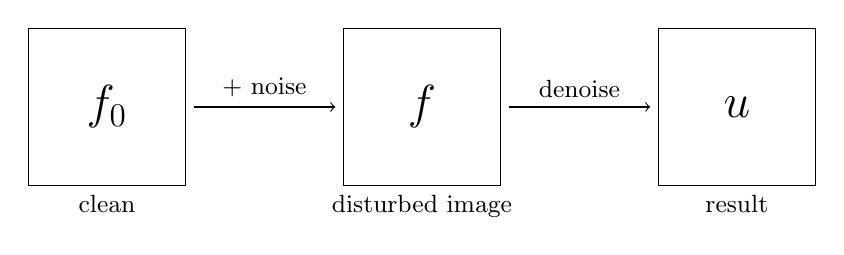
\begin{tikzpicture}
                \draw (0,0) rectangle (2,2);
                \draw (1,0) node[below] {\small clean};
                \draw (1,1) node[] {\LARGE $f_0$};
                \draw[->] (2.1,1) -- node[above] {\small $+$ noise} (3.9,1);
                \draw (4,0) rectangle (6,2);
                \draw (5,0) node[below] {\small disturbed image};
                \draw (5,1) node[] {\LARGE $f$};
                \draw[->] (6.1,1) -- node[above] {\small denoise} (7.9,1);
                \draw (8,0) rectangle (10,2);                
                \draw (9,0) node[below] {\small result};
                \draw (9,1) node[] {\LARGE $u$};
            \end{tikzpicture}
        \end{center}

        The quality of the denoised image $u$ compared to the original image $f_0$ is described by norms.
        \[\norm{f-f_0}, \text{noise}\]
        \[\norm{u-f_0}, \text{\mim{absolute error}}\]
        \[\frac{\norm{u-f_o}}{\norm{f-f_0}}, \text{\mim{relative error} compared to the noise}\]
        \[\frac{\norm{u-f_o}}{\norm{f_0}}, \text{relative error compared to the signal}\]
        
        Typically the chosen norm is:
        \[\norm{f} = \norm{f}_2 = \sqrt{\int_{\Omega} \abs{f(x)}^2 dx}\]
        or in the discrete:
        \[\norm{f}_2=\sqrt{\sum_{x \in \Omega} \abs{f(x)}^2}\]

        Closely connected is the \mim{Signal to noise ratio} (SNR):
        \[log(\underbrace{\frac{\norm{f_0}_2}{\norm{u-f_0}_2}}_{\in \ [1,\infty)}) \in [0,+\infty), \text{ where $0$ is bad and $+\infty$ is good.}\]
    \subsection{smoothing filter}
        Idea: (to simplify in 1D)
        \begin{center}
            \begin{tikzpicture}
                \draw (0,0) node[left] {$f_0$:};
                \draw[thick] plot [smooth, tension = 0.7] coordinates {(0,0) (1.75,1.5) (3.5,0.5) (6,2) (9,0) (11,0.5)};
                \draw[->,thick] (-0.3,-0.5) -- node[left] {noise} (-0.3,-2);
                \draw (0,-2.5) node[left] {$f$:};                
                \draw[thick, name path = P2,shift = {(0,-2.5)}] plot [smooth, tension = 0.7] coordinates {(0,0) (1.75,1.5) (3.5,0.5) (6,2) (9,0) (11,0.5)};
                \draw[name path = P1, draw = none] (0,-1.1) -- (3,-1.1);
                \draw[name intersections={of = P1 and P2},red,thick]
                (intersection-1) edge[bend right] ++(0.3,0.5) ++(0.3,0.5) edge[bend right] (intersection-2);
                \draw[name path = P3,draw = none] (3,-2.3) -- (5,-1.2);
                \draw[name intersections={of = P3 and P2},red,thick]
                (intersection-1) edge[bend left] ++(0.3,-0.3) ++(0.3,-0.3) edge[bend left] (intersection-2);
                \draw[] (2,-0.9) -- ++(0.5,-0.1) node[right] {\small disturbances} (3.5,-2.1) -- ++(-0.5,0.9);
                \draw (0,-5) node[left] {$f$:};
                \draw[thick, name path = P4,shift = {(0,-5)}] plot [smooth, tension = 0.7] coordinates {(0,0) (1.75,1.5) (3.5,0.5) (6,2) (9,0) (11,0.5)};
                \draw[name path = P5, shift = {(0,-2.5)}, draw = none] (0,-1.1) -- (3,-1.1);
                \draw[name intersections={of = P4 and P5},red,thick]
                (intersection-1) edge[bend right] node[black,pos=0] {\small \textbullet} ++(0.3,0.5) ++(0.3,0.5) edge[bend right] node[black,pos=1] {\small \textbullet}  node[black,pos=0] {\small \textbullet} (intersection-2);
                \draw[name path = P6, shift = {(0,-2.5)}, draw = none] (3,-2.3) -- (5,-1.2);
                \draw[name intersections={of = P4 and P6},red,thick]
                (intersection-1) edge[bend left] node[black,pos=0] {\small \textbullet} ++(0.3,-0.3) ++(0.3,-0.3) edge[bend left] node[black,pos=1] {\small \textbullet}  node[black,pos=0] {\small \textbullet} (intersection-2);
                \draw[decorate,decoration={brace,amplitude=2pt,mirror}] (1.4,-3.7) -- (2.2,-3.7);
                \draw[thick] (1.8,-3.8) -- (1.8,-4.3) node[below] {\small \framebox{average}};
                \draw[->,thick,double] (1.6,-5) -- (0.4,-5);
                \draw[->,thick,double] (2,-5) -- (3.2,-5);
                \draw[->,thick] (1.8,-5.1) -- (1.8,-5.7);
                \draw (0,-7.5) node[left] {$u$:};
                \draw[->,thick] (-0.3,-5.5) -- node[left] {denoising} (-0.3,-7);
                \draw[thick, name path = P7,shift = {(0,-7.5)}] plot [smooth, tension = 0.7] coordinates {(0,0) (1.75,1.5) (3.5,0.5) (6,2) (9,0) (11,0.5)};
                \draw[name path = P8, shift = {(0,-5)}, draw = none] (0,-1.2) -- (3,-1.2);
                \draw[name intersections={of = P7 and P8},red,thick]
                plot [smooth,tension=0.7] coordinates {(intersection-1) ($(intersection-1) + (0.5,0.35)$) (intersection-2)};
                \draw[name path = P9, shift = {(0,-5)}, draw = none] (3,-2.25) -- (5,-1.15);
                \draw[name intersections={of = P7 and P9},red,thick]
                plot [smooth,tension=0.7] coordinates {(intersection-1) ($(intersection-1) + (0.45,0.05)$) (intersection-2)};
            \end{tikzpicture}
        \end{center}

        \begin{equation} \label{eq:5.1}
            u(k):=\alpha \cdot f(k-1) + \beta \cdot f(k) + \gamma \cdot f(k+1)
        \end{equation}
        where:
        \begin{equation} \label{eq:5.2}
            \alpha + \beta + \gamma = 1
        \end{equation}

        More precisely \eqref{eq:5.1} means:
        
        \begin{center}
            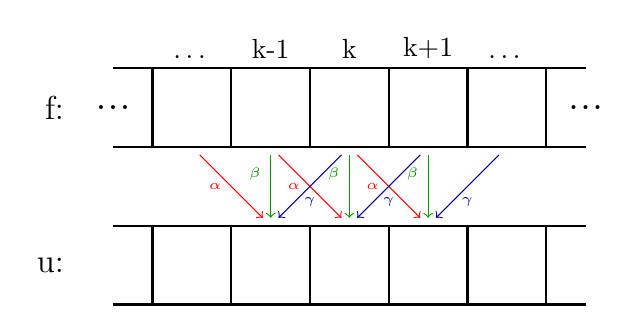
\begin{tikzpicture}
                \draw (0,-0.5) node[left] {\large f:};
                \draw[thick] (0.5,0) grid (6.5,-1);
                \draw (0.5,-0.5) node {\LARGE ...};
                \draw (6.5,-0.5) node {\LARGE ...};
                \draw (1.5,0) node[above] {\dots};
                \draw (2.5,0) node[above] {k-1};
                \draw (3.5,0) node[above] {k};
                \draw (4.5,0) node[above] {k+1};
                \draw (5.5,0) node[above] {\dots};

                \draw[->,red] (1.6,-1.1) -- node[left] {\tiny $\alpha$} (2.4,-1.9);
                \draw[->,red] (2.6,-1.1) -- node[left] {\tiny $\alpha$} (3.4,-1.9);
                \draw[->,red] (3.6,-1.1) -- node[left] {\tiny $\alpha$} (4.4,-1.9);
                \draw[->,black!40!green] (2.5,-1.1) -- node[left, pos = 0.3] {\tiny $\beta$} (2.5,-1.9);
                \draw[->,black!40!green] (3.5,-1.1) -- node[left, pos = 0.3] {\tiny $\beta$} (3.5,-1.9);
                \draw[->,black!40!green] (4.5,-1.1) -- node[left, pos = 0.3] {\tiny $\beta$} (4.5,-1.9);
                \draw[->,black!40!blue] (3.4,-1.1) -- node[right, pos = 0.75] {\tiny $\gamma$} (2.6,-1.9);
                \draw[->,black!40!blue] (4.4,-1.1) -- node[right, pos = 0.75] {\tiny $\gamma$} (3.6,-1.9);
                \draw[->,black!40!blue] (5.4,-1.1) -- node[right, pos = 0.75] {\tiny $\gamma$} (4.6,-1.9);

                \draw (0,-2.5) node[left] {\large u:};
                \draw[thick] (0.5,-2) grid (6.5,-3);
            \end{tikzpicture}
        \end{center}

        \begin{center}
            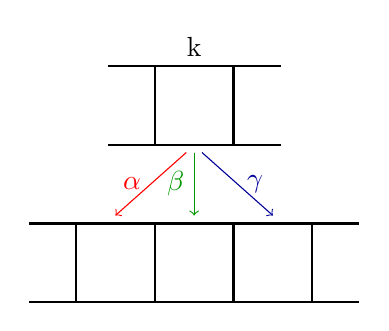
\begin{tikzpicture}
                \draw (0.5,0) node[above] {k};
                \draw[thick] (-0.6,0) grid (1.6,-1);
                \draw[->,red] (0.4,-1.1) -- node[left] {$\alpha$} (-0.5,-1.9);
                \draw[->,black!40!green] (0.5,-1.1) -- node[left] {$\beta$} (0.5,-1.9); 
                \draw[->,black!40!blue] (0.6,-1.1) -- node[right] {$\gamma$} (1.5,-1.9); 
                \draw[thick] (-1.6,-2) grid (2.6,-3);
            \end{tikzpicture}
        \end{center}

		With \eqref{eq:5.1} there is a mapping $f \mapsto u$, we write
		\[u = m \boxast f, \ \text{this is called \mim{Correlation}.}\]%TODO is it really correlation?
		where:
        \begin{equation}\label{eq:5.3}
            \framebox{$\displaystyle (m \boxast f)(k) = \sum_{i \in supp(m)} m(i) f(k+i)$}
        \end{equation}
        and:
        \begin{center}
            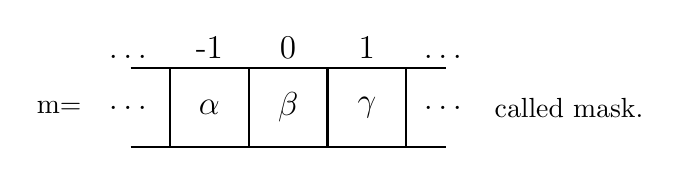
\begin{tikzpicture}
                \draw (0,0.5) node[left] {m=};
                \draw[thick] (0.5,0) grid (4.5,1);
                \draw (0.5,0.5) node {\large \dots};
                \draw (1.5,0.5) node {\large $\alpha$};
                \draw (2.5,0.5) node {\large $\beta$};
                \draw (3.5,0.5) node {\large $\gamma$};                
                \draw (4.5,0.5) node {\large \dots};
                \draw (0.5,1) node[above] {\large \dots};
                \draw (1.5,1) node[above] {\large -1};
                \draw (2.5,1) node[above] {\large 0};
                \draw (3.5,1) node[above] {\large 1};                
                \draw (4.5,1) node[above] {\large \dots};
                \draw (5,0.5) node[right] {called \mim{mask}.};
            \end{tikzpicture}
        \end{center}

        If you set $j:= k + i$ in \eqref{eq:5.1}, then $i=j-k$, which means:
        \begin{equation}\label{eq:5.4}
            \framebox{$\displaystyle (m \boxast f)(k) = \sum_{i \in supp(m)} m(j-k) f(j)$}
        \end{equation}

        To apply the mapping onto the boundary the image is reflected, in 1D:
        \begin{center}
            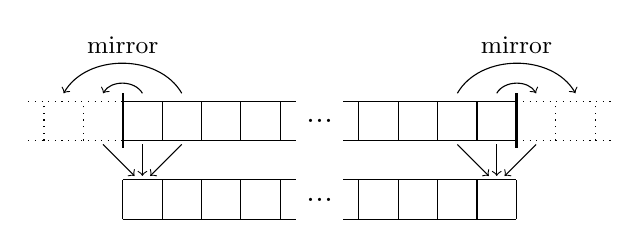
\begin{tikzpicture}
                \draw[step = 0.5] (0,0) grid (2.2,-0.5);
                \draw (2.5,-0.25) node {\large ...};
                \draw[step = 0.5] (2.8,0) grid (5,-0.5);
                \draw[thick] (0,0.1) -- (0,-0.6);
                \draw[thick] (5,0.1) -- (5,-0.6);
                \draw[step = 0.5, dotted] (0,0) grid (-1.2,-0.5);
                \draw[step = 0.5, dotted] (5,0) grid (6.2,-0.5);
                \draw[] (0.25,0.1) edge[bend right = 60, ->] (-0.25,0.1);
                \draw[] (0.75,0.1) edge[bend right = 60, ->] node[above] {\small mirror} (-0.75,0.1);
                \draw[] (4.75,0.1) edge[bend left = 60, ->] (5.25,0.1);
                \draw[] (4.25,0.1) edge[bend left = 60, ->] node[above] {\small mirror} (5.75,0.1);
                \draw[step = 0.5] (0,-1) grid (2.2,-1.5);
                \draw (2.5,-1.25) node {\large ...};
                \draw[step = 0.5] (2.8,-1) grid (5,-1.5);
                \draw[->] (0.25,-0.55) -- (0.25,-0.95);
                \draw[->] (-0.25,-0.55) -- (0.15,-0.95);
                \draw[->] (0.75,-0.55) -- (0.35,-0.95);
                \draw[->] (4.75,-0.55) -- (4.75,-0.95);
                \draw[->] (4.25,-0.55) -- (4.65,-0.95);
                \draw[->] (5.25,-0.55) -- (4.85,-0.95);
            \end{tikzpicture}
        \end{center}

        in 2D:

        \begin{center}
            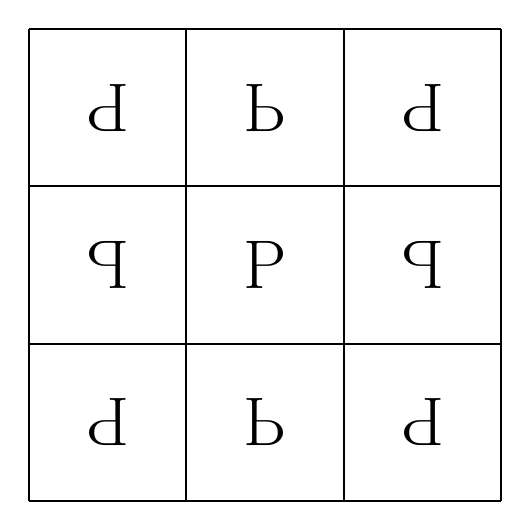
\begin{tikzpicture}
                \draw[step =2, thick] (0,0) grid (6,6);
                \draw (3,3) node {\Huge P};
                \draw (1,1) node[rotate = 180] {\Huge P};
                \draw (5,1) node[rotate = 180] {\Huge P};
                \draw (1,5) node[rotate = 180] {\Huge P};
                \draw (5,5) node[rotate = 180] {\Huge P};
                \draw (3,5) node[yscale=-1,xscale=1] {\Huge P};
                \draw (5,3) node[rotate = 180,yscale=-1,xscale=1] {\Huge P};
                \draw (1,3) node[rotate = 180,yscale=-1,xscale=1] {\Huge P};
                \draw (3,1) node[yscale=-1,xscale=1] {\Huge P};
            \end{tikzpicture}
        \end{center}

        Formula \eqref{eq:5.4} might remind one of the \mim{convolution}:
        \begin{equation}\label{eq:5.5}
            \framebox{$\displaystyle (g * f)(k) = \sum_{j \in \Z} g(\underbrace{k-j}_{\text{Difference to \eqref{eq:5.4}}}) \cdot f(j)$}
        \end{equation}

        If you set $g(i) := m(-i) =: \tilde m(i)$, which corresponds to a reflection of the Mask, then
        \[m \boxast f = g * f = \tilde m * f\]

        Properties of the convolution:
        \begin{enumerate}
            \item $(f * g) * h = f * (g* h)$, Associativity
            \item $f*g=g*f$, Commutativity
            \item $\tilde f * \tilde g = \widetilde{f * g}$, Compatibility with reflection
        \end{enumerate}
        
        Properties of the correlation:
        \begin{enumerate}
            \item $f \boxast (g \boxast h) = \tilde f * ( \tilde g* h) \overset{\framebox{\small 1}}{=} ( \tilde f * \tilde g) * h \overset{\framebox{\small 3}}{=} (\widetilde{f * g}) * h = (f * g) \boxast h \neq (f \boxast g) \boxast h$, not associative!
            \item $f \boxast g = \tilde f * g \overset{\framebox{\small 2}}{=} g * \tilde f = \tilde{\tilde g} * \tilde f \overset{\framebox{\small 3}}{=} \widetilde{(\tilde g * f)} = \widetilde{g \boxast f} \neq g \boxast f$, not commutative!
            \item $\tilde f \boxast \tilde g = \tilde{\tilde f} * \tilde g \overset{\framebox{\small 3}}{=} \widetilde{(\tilde f * g)} = \widetilde{f \boxast g}$, Compatibility with reflection
        \end{enumerate}
%\chapter{6.Kantenerkennung}


\section{\mim{Gradientenfilter}}
Wir suchen Stellen $\x$ mit großem Gradienten:
\[\nabla u(\x) = \srmatrix{\frac{\partial u}{\partial x}(\x)\\\frac{\partial u}{\partial y}(\x)}\]
Approximation der Gradienten über zentrale Differenzen:
\begin{equation}\label{eq:6.1}
    \frac{\partial}{\partial x} \approx \frac{1}{2} \begin{tabular}{|c|c|c|}\hline
        -1 & 0 & 1\\
        \hline
    \end{tabular} \text{ bzw. } \frac{\partial}{\partial y} \approx \frac{1}{2} \begin{tabular}{|c|c|c|}\hline
        -1\\
        \hline
        0\\
        \hline
        1\\
        \hline
    \end{tabular}
\end{equation}

Um Rauschen zu verringern wird auch ein entrauschen Filter simultan angewendet:

\begin{center}
    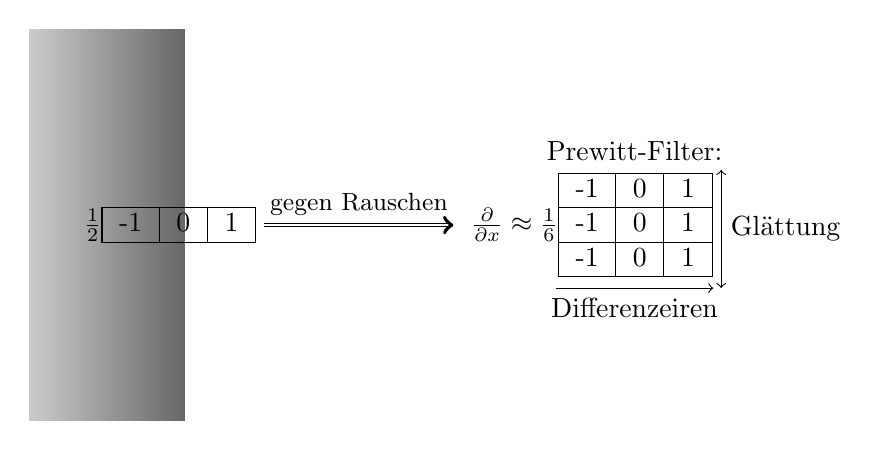
\begin{tikzpicture}
        \draw[left color=black!20!white, right color=black!60,color=white] (0,0) rectangle (2,5);
        \draw (1.8,2.5) node[] {$\frac{1}{2} \begin{tabular}{|c|c|c|}\hline
            -1 & 0 & 1\\
            \hline
        \end{tabular}$};
        \draw[->,double] (3,2.5) -- node[above] {\small gegen Rauschen}(5.4,2.5);
        \draw (5.5,2.5) node[right] {$\frac{\partial }{\partial x} \approx  \frac{1}{6} \begin{tabular}{|c|c|c|}\hline
            -1 & 0 & 1\\
            \hline
            -1 & 0 & 1\\
            \hline
            -1 & 0 & 1\\
            \hline
        \end{tabular}$};
        \draw[->] (6.7,1.7) -- node[below] {Differenzeiren} (8.7,1.7);
        \draw[<->] (8.8,3.2) -- node[right] {Glättung} (8.8,1.7);
        \draw (7.7,3.2) node[above] {\mim{Prewitt-Filter}:};
    \end{tikzpicture}
\end{center}

Alternative: $\frac{\partial }{\partial x} \approx \frac{1}{2} \begin{tabular}{|c|c|c|}\hline
    -1 & 0 & 1\\
    \hline
\end{tabular} \boxast \frac{1}{4}\begin{tabular}{|c|c|c|}\hline
    -1\\
    \hline
    0\\
    \hline
    1\\
    \hline
\end{tabular} = \frac{1}{8} \begin{tabular}{|c|c|c|}\hline
-1 & 0 & 1\\
\hline
-2 & 0 & 2\\
\hline
-1 & 0 & 1\\
\hline
\end{tabular}=:D_x$, genannt \mim{Sobel-Filter}.
Eine stärkere Glättung kann mittels anderer vertikaler Filter mit Binomialkoeffizienten erzeilt werden.\\

Entsprechen wird $\frac{\partial }{\partial y} D_y:=D_x^T$ definiert.\\

\begin{equation}\label{eq:6.2}
    \nabla u(\x) = \srmatrix{\frac{\partial u}{\partial x}(\x)\\\frac{\partial u}{\partial y}(\x)} \approx \srmatrix{(D_x \boxast u)(\x)\\ (D_y \boxast u)(\x)}
\end{equation}

Zur Erinnerung der Gradienten steht senkrecht auf Kanten und zeigt in Richtung heller (hoher) Werte, die Intensität wird beschrieben von $\abs{\nabla u(\x)}$, also dem Betrag des Gradienten.

Ein typischer Algorithmus kann etwa folgende Form annehmen:
\begin{enumerate}
    \item Gradienten mittels Prewitt oder Sobel approximieren und Richtung auf Vielfache von $45^\circ$ runden.
    \item \mim{Non-maximum suppression} (edge thinning). Da es potentiell viele Punkte mit hoher Steigung gibt kann es dazu kommen, dass Kanten sehr breit werden, dieses wird durch das edge thinning verhindert.

\begin{center}
    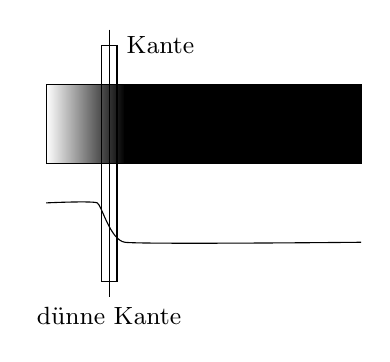
\begin{tikzpicture}
        \draw[left color=white, right color=black] (0,0) rectangle (1,1);
        \draw[fill] (1,0) rectangle (4,1);
        \draw[shift={(0,-1)}] plot [smooth, tension = 0.2] coordinates {(0,0.5) (0.65,0.5) (1,0) (4,0)};
        \draw (0.7,1.5) rectangle (0.9,-1.5);
        \draw (0.9,1.5) node[right] {\small Kante};
        \draw (0.8,1.7) -- (0.8,-1.7) node[below] {\small dünne Kante};
    \end{tikzpicture}
\end{center}

Mathematisch: $\x$ wird Kantenpunkt falls:
\[\abs{\nabla u(\x)} \leq max(\abs{\nabla u(\x_+)},\abs{\nabla u(\x_-)})\]
wobei $\x_+$ und $\x_-$ Vorgänger und Nachfolger von $\x$ in Gradientenrichtung sind.
\item Kandidat $\x$ wird Kantenpunkt, falls:
\begin{center}
    
\begin{tikzpicture}
        \draw (0,0) -- (11,0);
        \draw[decorate,decoration={brace,amplitude=5pt}] (0.1,0.1) -- node[above] {\small Kein Kantenpunkt} (2.95,0.1);
        \draw[decorate,decoration={brace,amplitude=5pt}] (3.05,0.1) -- node[above] {\small Ja, falls Nachbar Kantenpunkt} (7.95,0.1);
        \draw[decorate,decoration={brace,amplitude=5pt}] (8.05,0.1) -- node[above] {\small Kantenpunkt} (10.95,0.1);
        \draw (3,0.2) -- (3,-0.2) node[below] {\small $t_1$};
        \draw (8,0.2) -- (8,-0.2) node[below] {\small $t_2$};
    \end{tikzpicture}
\end{center}
wobei $t_1, \ t_2$ thresholds sind.\\
$\x$ ist also ein Kantenpunkt, falls $\abs{\nabla u(\x)} \geq t_2$ oder $\left( \abs{\nabla u(\x)} \in [t_1,t_2] \text{ und $\x$ ist Nachbar eines Kantenpunktes}  \right)$.
Dieses wird \mim{hysteresis thresholding} genannt und verhindert \mim{Abreißen} von Kantenzügen.
\end{enumerate}

Die am häufigsten verbreitete Version von 1) -3) ist der \mim{Canny-Algorithmus} (1986).

Matlab:
\begin{lstlisting}
    BWimg=edge(u,'canny',[t_1, t_2],sigma);
\end{lstlisting}

\begin{enumerate}
    \item[BWimg:] Binärbild
    \item[u:] Graustufenbild
    \item[canny:]Algorithmus
    \item[$t_1, \ t_2$:] Sind gewählt wie oben
    \item[sigma:] Parameter für den Gaußkern aus 1)
\end{enumerate}

\section{Die zweite Ableitung}

Zunächst in 1D:
%Wenn jemand eine bessere Idee hat, kann er das gerne aufräumen.
\begin{center}
    \begin{tikzpicture}
        \draw[dotted] (-0.5,0) node[left] {\small $u$:}-- (8.5,0);
        \draw[scale=1,domain=-2:0,smooth,variable=\x,shift ={(2,0)}] plot ({\x},{(e^((-(\x)^2)/(0.2))}) -- (4,1) [scale=1,domain=0:2,smooth,variable=\x,shift ={(4,0)}] plot({\x},{(e^((-(\x)^2)/(0.2))});

        \draw[dotted] (-0.5,-2) node[left] {\small $u'$:}-- (8.5,-2);
        \draw[scale=1,domain=-1.5:1,smooth,variable=\x,shift ={(1.5,-2)}] plot ({\x},{(e^((-(\x)^2)/(0.05))}) -- (4,0) [scale=1,domain=-1:1.5,smooth,variable=\x,shift ={(5,0)}] plot({\x},{-(e^((-(\x)^2)/(0.05))});

        \draw[dotted] (-0.5,-4) node[left] {\small $u''$:}-- (8.5,-4);
        \draw[scale=1,domain=-1.5:1,smooth,variable=\x,shift ={(1.5,-4)}] plot ({\x},{-5*\x*(e^((-(\x)^2)/(0.05))}) -- (4,0) [scale=1,domain=-1:1.5,smooth,variable=\x,shift ={(5,0)}] plot({\x},{5*\x*(e^((-(\x)^2)/(0.05))});

        \draw(1.5,1.2)--(1.5,-4.5);
        \draw(6.5,1.2)--(6.5,-4.5);
        \draw[] (1.5,0.2865) node[circle,fill,inner sep=1pt] {};
        \draw (6.5,0.2865) node[circle,fill,inner sep=1pt] {};
        \draw (1.5,-1.02) node[circle,fill,inner sep=1pt] {};
        \draw (6.5,-2.98) node[circle,fill,inner sep=1pt] {};
        \draw (1.5,-4) node[circle,fill,inner sep=1pt] {};
        \draw (6.5,-4) node[circle,fill,inner sep=1pt] {};
    \end{tikzpicture}
\end{center}

Test für kantenpunkte $u''(\x) = 0$ und $\abs{u'(\x)}>$ threshold.\\
Wichtig: Vorglätten!, da die 2. Ableitung noch anfälliger gegenüber Rauschen als die 1. Ableitung ist.\\
\ \\
In 2D. Laplace Operator $\Delta u = \frac{\partial^2 u}{\partial^2 x} + \frac{\partial^2 u}{\partial^2 y}$ (Richtungsunabhängige Messung der 2. Ableitung)\\
Vorglätten: $\Delta (G * u) = (\Delta G)*u$, wobei $\Delta G$ vorher berechnet werden kann.

In 1D:

\begin{center}
    \begin{tikzpicture}
        \draw (0,0.2) node[left] {$G:$};
        \draw[scale=1,domain=-1.5:1.5,smooth,variable=\x,shift ={(2,0)}] plot ({\x},{(e^((-(\x)^2)/(0.2))});
        \draw (4.5,0.2) node[left] {$\Delta G:$};
        \draw[scale=0.5,domain=-4:4,smooth,variable=\x,shift ={(13,0)}] plot ({\x},{(\x*\x*(e^((-(\x)^2)/(2))) - (e^((-(\x)^2)/(2))});
    \end{tikzpicture}
\end{center}

In 2D:
\def\centerx{2}
\def\centery{-1}
\begin{center}
    \begin{tikzpicture}
    \pgfplotsset{
        colormap name=\chsixgaussfigsampleColor,
    }
        \begin{axis}[hide axis,scale=-1.75,name=plot1,samples=60]
            \addplot3[surf,domain=-2:6,domain y=-3.7:3.7,samples=\chsixgaussfigsampleone]
                {exp(-( (x-\centerx)^2 + (y-\centery)^2)/3 )};
         \end{axis}
            \draw[->] (6,1.5)--(7,1.5);
            \draw (1.5,0) node[left] {\Large $G$};
            \draw (7.5,0) node[left] {\Large $\Delta G$};
        \begin{axis}[hide axis,scale=0.75,at={(8cm,1cm)}, anchor=center]
            \addplot3[surf,domain=-3:3,domain y=-5:5,samples=\chsixgaussfigsampleTwo]
            {x^2*exp(- x^2/2 - y^2/2) - 2*exp(- x^2/2 - y^2/2) + y^2*exp(- x^2/2 - y^2/2)};
        \end{axis}
    \end{tikzpicture}
\end{center}

Dieses wird \mim{Laplacian of Gaußian method} genannt.\\
Matlab:
\begin{lstlisting}
    BWimg=edge(u,'log',thresh,sigma);
\end{lstlisting}
$\Rightarrow$ alle $\x \in \Omega$ mit:
\begin{enumerate}
    \item[] $\Delta (G_{sigma} * u)(\x) \approx u$, nicht auf Gleichheit sondern auf Vorzeichenwechsel testen.
    \item[und:] $\abs{\nabla(G_{sigma}) * u}>\text{thresh}$
\end{enumerate} 

%\include{Chapters/7.Schärfen_und_Entfalten}
%\chapter{8.Restauration und Inpainting}
  Problem: Lücken im Bild, etwa 

  \begin{enumerate}
    \item Kratzer
    \item Scannerzeile kaputt
    \item Defekt in der Kamera
    \item Bewusst entferntes Objekt
  \end{enumerate}
  sollen sinvoll und unauffällig geschlossen werden.

  Sei $f: \Omega \to F$ unser Bild jedoch mit Defekt, d.h. fehlenden Funktionswerten in $D \subset \Omega$.

  \begin{enumerate}
    \item[1. Fall:] Jeder Punkt aus $D$ hat Nachbarn in $\Omega \backslash D$.\\
    $\Rightarrow$ Lücken mittels Interpolation aus benachbarten Werten in $\Omega \backslash D$ schließen.
    \item[2. Fall:] $D$ hat innere Punkte. Diesen Fall werden wir im folgenden näher betrachten.
  \end{enumerate}

  \section{Frequenzraum-Ansatz}
    Zur Illustration in 1D:
    \begin{center}
      \begin{tikzpicture}[scale = 1.3]
        \draw (0,0) -- (8,0);
        \draw[thick] plot [smooth, tension = 0.8] coordinates {(1,1) (2,1.2) (3,1) (4,1.3) (5,1.7) (6,1.5) (7,2)};
        \draw[fill,color=white] (3,0.5) rectangle (5,2);
        \draw (1,-0.1) -- (1,0.1);
        \draw (3,-0.1) -- (3,0.1);
        \draw (5,-0.1) -- (5,0.1);
        \draw (7,-0.1) -- (7,0.1);
        \draw (5.3,-0.1) -- (5.3,0.1);
        \draw (2.7,-0.1) -- (2.7,0.1);
        \draw[decorate,decoration={brace,amplitude=2pt,mirror}] (1,-0.5) -- node[below] {\small $\Omega$} (7,-0.5);
        \draw[thick, line width =0.6mm] (3,0) -- node[below] {\small $D$} (5,0);
        \draw[decorate,decoration={brace,amplitude=2pt,mirror}] (2.7,-0.15) -- node[below] {\small $u$} (3,-0.15);
        \draw[decorate,decoration={brace,amplitude=2pt,mirror}] (5,-0.15) -- node[below] {\small $u$} (5.3,-0.15);
      \end{tikzpicture}
    \end{center}
    Betrachte Umgebung $u \subset \Omega \backslash D$ und errechne den Mittelwert:
    \[ m:= \frac{1}{\abs{u}} \int_u f(x) dx\]
    von $f$ auf $u$.
    
    \textbf{Algorithmus:}
    \ \\
    \begin{tikzpicture}
        \node at (5, 10) {
    {\begin{varwidth}{\linewidth}\begin{enumerate}
        \item[\texttt{[1]}] Initialisiere $f$ auf $D$ mittels konstanter Funktion $m$:
          \begin{center}
            \begin{tikzpicture}
              \draw (0,0) -- (8,0);
              \draw[thick] plot [smooth, tension = 0.8] coordinates {(1,1) (2,1.2) (3,1) (4,1.3) (5,1.7) (6,1.5) (7,2)};
              \draw[fill,color=white] (3,0.5) rectangle (5,2);
              \draw (1,-0.1) -- (1,0.1);
              \draw (3,-0.1) -- (3,0.1);
              \draw (5,-0.1) -- (5,0.1);
              \draw (7,-0.1) -- (7,0.1);
              \draw[dashed,thick,red,line width=0.4mm] (3,1) -- (3,1.4) -- (5,1.4) -- (5,1.7);
              \draw[thick, line width =0.6mm] (3,0) -- node[below] {\small $D$} (5,0);
              \draw[<-] (3.05,1.2) -- (6,0.5);
              \draw[<-] (5.05,1.6) -- (6,0.5) node[right] {\small Sprünge};
            \end{tikzpicture}
          \end{center}
          $\Rightarrow$ Sprünge am Rand von $D$.\\
          Idee: Sprünge $\widehat =$ hochfrequente Anteile $\Rightarrow$ wende Tiefpass filter an.
        \item[\texttt{[2]}] $ f \xrightarrow{\F} \hat f \xrightarrow{\text{Lösche hohe Frequenzen}} \hat g \xrightarrow{\F^{-1}}g$
          \begin{center}
            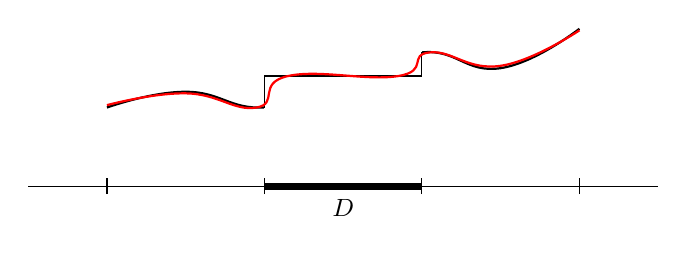
\begin{tikzpicture}
              \draw (0,0) -- (8,0);
              \draw[thick] plot [smooth, tension = 0.8] coordinates {(1,1) (2,1.2) (3,1) (4,1.3) (5,1.7) (6,1.5) (7,2)};
              \draw[fill,color=white] (3,0.5) rectangle (5,2);
              \draw (1,-0.1) -- (1,0.1);
              \draw (3,-0.1) -- (3,0.1);
              \draw (5,-0.1) -- (5,0.1);
              \draw (7,-0.1) -- (7,0.1);
              \draw[] (3,1) -- (3,1.4) -- (5,1.4) -- (5,1.7);
              \draw[thick, line width =0.9mm] (3,0) -- node[below] {\small $D$} (5,0);
              \draw[thick,red] plot [smooth, tension = 0.8] coordinates {(1,1.03) (2,1.18) (2.9,1) (3.3,1.4) (4.7,1.4) (5.1,1.7) (6,1.53) (7,1.98)};
            \end{tikzpicture}
          \end{center}
        \item[\texttt{[3]}] Ersetze $f$ \underline{innerhalb} von $D$ durch $g$.
          \begin{center}
            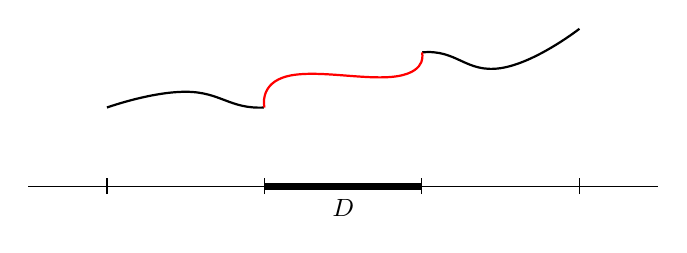
\begin{tikzpicture}
              \draw (0,0) -- (8,0);
              \draw[thick] plot [smooth, tension = 0.8] coordinates {(1,1) (2,1.2) (3,1) (4,1.3) (5,1.7) (6,1.5) (7,2)};
              \draw[fill,color=white] (3,0.5) rectangle (5,2);
              \draw (1,-0.1) -- (1,0.1);
              \draw (3,-0.1) -- (3,0.1);
              \draw (5,-0.1) -- (5,0.1);
              \draw (7,-0.1) -- (7,0.1);
              \draw[thick, line width =0.9mm] (3,0) -- node[below] {\small $D$} (5,0);
              \draw[thick,red] plot [smooth, tension = 0.8] coordinates {(3,1) (3.3,1.4) (4.7,1.4) (5,1.7)};
            \end{tikzpicture}
          \end{center}
      \end{enumerate}\end{varwidth}}};
      \draw[->,thick] (0,5.5) -- (-1,5.5) -- node[sloped,above]  {Iteriere} node[sloped,below] {\footnotesize Abbruch falls $\norm{f-g}< \ threshold$} (-1,10.9) -- (-0.5,10.9);
    \end{tikzpicture}
    
  \section{PDE-Transport-Diffusions-Ansatz}
    \begin{minipage}[c]{0.25\linewidth}
      \begin{center}
        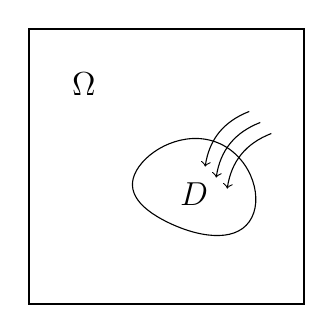
\begin{tikzpicture}[scale=0.7]
          \draw[thick] (0,0) rectangle (5,5);
          \draw plot [smooth cycle,tension=1] coordinates {(2.5,1.5) (2,2.5) (3.5,2.9) (4,1.5)};
          \draw (3,2) node[] {\large $D$};
          \draw (1,4) node[] {\large $\Omega$};
          \draw[<-] (3.2,2.5) to[bend left] (4,3.5);
          \draw[<-] (3.4,2.3) to[bend left] (4.2,3.3);
          \draw[<-] (3.6,2.1) to[bend left] (4.4,3.1);
        \end{tikzpicture}
      \end{center}
    \end{minipage}
    \hfill
    \begin{minipage}[c]{0.65\linewidth}
        \begin{enumerate}
          \item[Idee:] Informationen aus $\Omega \backslash D$ nach $D$ ''hineintragen''.
          \item[Referenzen:] \begin{enumerate}
            \item[\textbullet] Weichert 1998
            \item[\textbullet] Bornemann \& März 2007
          \end{enumerate}
        \end{enumerate}
    \end{minipage}
    \ \\
    \ \\
    \hfill\\
    \textbf{Skalierung der Diffusion:}
    \[\frac{\partial u}{\partial t} = div(M \nabla u)\]
    \[\text{mit } M = \srmatrix{ | & |\\ v_1 & v_2\\ | & |} \mat{\lambda_1 & \ \\ & \lambda_2} \srmatrix{- & v_1^T & -\\ \\- & v_2^T & -} \in R^{2 \times 2}\]
    Wobei $v_1 \perp v_2$ die Eigenvektoren des sogenannten \underline{doppelt geglätteten Strukturrensors} \index{doppelt geglätteter Strukturrensor}
    \[J= G_\rho * \biggl[ \underbrace{\srmatrix{| \\ \nabla (G_\sigma * u)\\ |}}_{2 \times 1} \cdot \underbrace{\srmatrix{- & \nabla^T(G_\sigma * u) & -}}_{1 \times 2} \biggr] \]
    sind.\\
    \begin{enumerate}
      \item[$\Rightarrow$] $v_1$ Richtung mit maximalem Kontrast mit EW $\mu_1$
      \item[] $v_2$ Richtung mit maximalem Kontrast mit EW $\mu_2$, genannt \mim{Kohärentsrichtung}.
      \item[] Hierbei ist $\mu_1 \geq \mu_2$.
    \end{enumerate}
    
    \begin{center}
        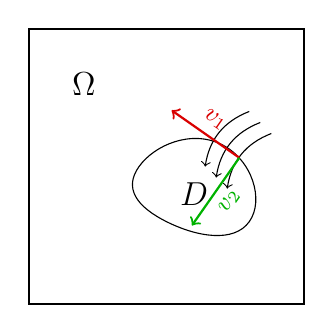
\begin{tikzpicture}[scale=0.7]
          \draw[thick] (0,0) rectangle (5,5);
          \draw plot [smooth cycle,tension=1] coordinates {(2.5,1.5) (2,2.5) (3.5,2.9) (4,1.5)};
          \draw (3,2) node[] {\large $D$};
          \draw (1,4) node[] {\large $\Omega$};
          \draw[<-] (3.2,2.5) to[bend left] (4,3.5);
          \draw[<-] (3.4,2.3) to[bend left] (4.2,3.3);
          \draw[<-] (3.6,2.1) to[bend left] (4.4,3.1);
          \draw[->,red!85!black,thick] (3.82,2.66) -- node[sloped,above] {\small $v_1$} ++(-215:1.5);
          \draw[->,green!70!black,thick] (3.82,2.66) -- node[sloped,below] {\small $v_2$} ++(-125:1.5);
        \end{tikzpicture}
      \end{center}
      
      Fälle:
      \begin{enumerate}
        \item[] 
        \begin{minipage}[c]{0.25\linewidth}
          $\mu_1 \gg \mu_2 \approx 0$
        \end{minipage}
        \begin{minipage}[c]{0.25\linewidth}
          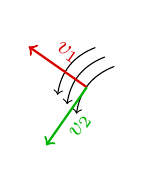
\begin{tikzpicture}[scale =0.6]
            \draw[<-] (3.2,2.5) to[bend left] (4,3.5);
            \draw[<-] (3.4,2.3) to[bend left] (4.2,3.3);
            \draw[<-] (3.6,2.1) to[bend left] (4.4,3.1);
            \draw[->,red!85!black,thick] (3.82,2.66) -- node[sloped,above] {\small $v_1$} ++(-215:1.5);
          \draw[->,green!70!black,thick] (3.82,2.66) -- node[sloped,below] {\small $v_2$} ++(-125:1.5);
          \end{tikzpicture}
        \end{minipage}
                \item[] 
        \begin{minipage}[c]{0.25\linewidth}
          $\mu_1 \approx \mu_2 \approx 0$
        \end{minipage}
        \begin{minipage}[c]{0.12\linewidth}
          
\begin{tikzpicture}[scale =0.6]
            \definecolor{left} {HTML}{001528}
            \draw[shading = axis,rectangle, left color=left!70!white, right color=left!60!white,shading angle=135, anchor=north,fill,draw=white] (0,0) rectangle (2,2);
          \end{tikzpicture}
        \end{minipage}
        \begin{minipage}[c]{0.3\linewidth}
          Lokal keine Struktur.
        \end{minipage}
        \item[] 
        \begin{minipage}[c]{0.25\linewidth}
          $\mu_1 \approx \mu_2 \gg 0$
        \end{minipage}
        \begin{minipage}[c]{0.12\linewidth}
          
\begin{tikzpicture}[scale =0.6]
            \definecolor{left} {HTML}{001528}
            \draw[shading = axis,rectangle, left color=left!20!white, right color=left!30!white,shading angle=135, anchor=north,fill,draw=white] (0,0) rectangle (2,2);
            \draw[line width = 0.8mm] (0,0) -- (2,0) -- (2,2);
          \end{tikzpicture}
        \end{minipage}
        \begin{minipage}[c]{0.3\linewidth}
          Kanten.
        \end{minipage}
      \end{enumerate}
      
      Die Werte $\lambda_1$ und $\lambda_2$ werden wie folgt gewählt:\\
      $\alpha \in (0,1)$ wird festgehalten.
      
      \begin{center}
        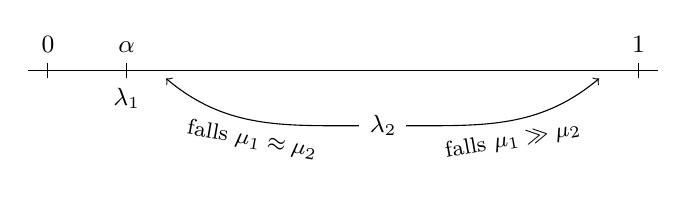
\begin{tikzpicture}[scale = 1]
            \draw[] (0,0) -- (8,0);
            \draw (0.25,-0.1) -- (0.25,0.1) node[above] {\small $0$};
            \draw (7.75,-0.1) -- (7.75,0.1) node[above] {\small $1$};
            \draw (1.25,-0.1) node[below] {\small $\lambda_1$} -- (1.25,0.1) node[above] {\small $\alpha$};
            \draw[->] (4.2,-0.7) to[out=180, in =-40] node[sloped,below] {\footnotesize falls $\mu_1 \approx \mu_2$} (1.75,-0.1);
            \draw[<-] (7.25,-0.1) to[in=0,out =-140] node[sloped,below] {\footnotesize falls $\mu_1 \gg \mu_2$} (4.8,-0.7) node[left] {\small $\lambda_2$};
          \end{tikzpicture}
      \end{center}
      
      \[\lambda_1 := \alpha, \ \lambda_2 := \alpha + (1 - \alpha)(1-g(\mu_1 - \mu_2))\]
      
      wobei $g$ wie bei Perona Malik gewählt wird, also:
      
      \[g(x)=\frac{1}{1 + \frac{s^2}{\kappa^2}}\]
      
      Dieses wird \mim{Kohärenz verstärkende Diffusion} genannt.
      
      \section{Variationsansatz}


        \begin{minipage}[c]{0.25\linewidth}
      \begin{center}
        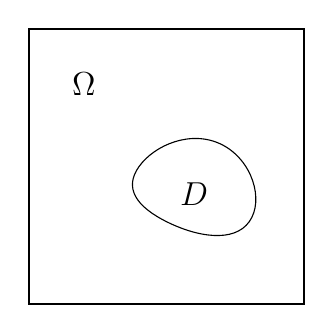
\begin{tikzpicture}[scale=0.7]
          \draw[thick] (0,0) rectangle (5,5);
          \draw plot [smooth cycle,tension=1] coordinates {(2.5,1.5) (2,2.5) (3.5,2.9) (4,1.5)};
          \draw (3,2) node[] {\large $D$};
          \draw (1,4) node[] {\large $\Omega$};
        \end{tikzpicture}
      \end{center}
    \end{minipage}
    \hfill
    \begin{minipage}[c]{0.5\linewidth}
        \begin{enumerate}
          \item[geg.:] $f$ auf $\Omega \backslash D$
          \item[ges.:] $u$ auf $\Omega$
          \item[Wunsch 1:] $u=f$ auf $\Omega \backslash D$
          \item[Wunsch 2:] $\norm{\nabla u}$ klein auf $\Omega$
        \end{enumerate}
    \end{minipage}\\
    \hfill\\ \hfill\\
    Daraus folgt:
    
    \[ J(u):= \norm{\nabla u}_2^2 \to \text{min} \]
    
    auf
    
    \[U:=\{u \in W^{1,2}(\Omega) : u|_{\Omega \backslash D} = f\} \]
    
    Angenommen, $u \in U$ minimiert $J$, dann folgt für beliebige $v \in W^{1,2} (\Omega)$ mit $v|_{\Omega \backslash D}=0$:
    
    \begin{align*}
      0 &= \underset{t \to 0}{lim} \frac{J(u+tv) - J(u)}{t} = \underset{t \to 0}{lim} \frac{1}{t} \int_\Omega ||\underbrace{\nabla(u+tv)(x)}_{\nabla u(x) + t \nabla v(x)}||^2 - \norm{\nabla u(x)}^2 dx\\
      &=\underset{t \to 0}{lim} \frac{1}{t} \int_\Omega \skprod{\nabla u(x) + t \nabla v(x)}{\nabla u(x) + t \nabla v(x)} - \skprod{\nabla u (x)}{\nabla u (x)} dx\\
      &=\underset{t \to 0}{lim} \frac{1}{t} \int_\Omega t^2 \norm{\nabla v(x)}^2 + 2 t \skprod{\nabla u(x)}{\nabla v(x)} dx =  \underset{t \to 0}{lim} \int_\Omega t \norm{\nabla v(x)}^2 + 2 \skprod{\nabla u(x)}{\nabla v(x)} dx\\
      &=2 \int_D \skprod{\nabla u(x)}{\nabla v(x)} dx \overset{\text{Greensche Formel}}{=} 2 \biggl( \overbrace{\int_{\delta D} \frac{\partial u}{\partial n} \underbrace{v(x)}_{0} ds(x)}^{0} - \int_D \Delta u(x) v(x) dx \biggr)\\
      &=2 \int_D \Delta u(x) v(x) dx \Rightarrow \nabla u =0 \text{ in } D
    \end{align*}

%\chapter{9.Segementierung}

\newcommand{\quo}[1] {
\glqq #1 \grqq
}

Dieses ist die Zerlegung eines Bildes in verschiedene Objekt.\\
Eine einfach methode hierfür ist das \mim{Historgramm thresholding}:
\begin{center}
  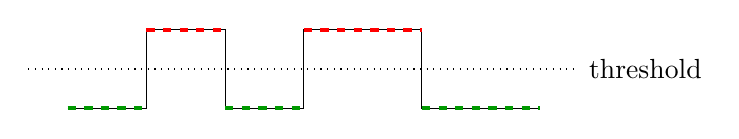
\begin{tikzpicture}
    \draw (1,0) -- (2,0) -- (2,1) -- (3,1) -- (3,0) -- (4,0) -- (4,1) -- (5.5,1) -- (5.5,0) -- (7,0);
    \draw[dotted] (0.5,0.5) -- (7.5,0.5) node[right] {threshold};
    \draw[line width=0.5mm,red,dashed] (2,1) -- (3,1);
    \draw[line width=0.5mm,red,dashed] (4,1) -- (5.5,1);
    \draw[line width=0.5mm,green!60!black,dashed] (1,0) -- (2,0);
    \draw[line width=0.5mm,green!60!black,dashed] (3,0) -- (4,0);
    \draw[line width=0.5mm,green!60!black,dashed] (5.5,0) -- (7,0);
  \end{tikzpicture}
\end{center}
So kann ein Bild in mehrere Objekte zerlegt werden.\\
Hierbei können jedoch diverse Probleme auftreten, die durch preprocessing vermindert werden sollten. Einige der preprocessing methoden sind:
\begin{enumerate}
  \item[-] Entrauschen $\nearrow$ 5.7
  \item[-] Farbraum optimal ausnutzen $\nearrow$ 3.2
  \item[-] \mim{Beleuchtungsausgleich}
\end{enumerate}
Dieser Beleuchtungsausgleich wurde nohc nicht vorher besprochen, das Problem:

\begin{center}
  \begin{tikzpicture}
    \draw (0,0) -- ++(20:1) -- ++(0,1) -- ++(20:1) -- ++(0,-1) -- ++(20:1) -- ++(0,1) -- ++(20:1.5) -- ++(0,-1) -- ++(20:1.5);
    \draw[dotted] (-0.5,1.5) -- (6,1.5) node[right] {threshold??};
  \end{tikzpicture}
\end{center}

Anstatt eines \quo{geraden} Bildes ist das Bild, etwa durch Beleuchtung, \quo{gekippt} und der Ansatz mittels Histogramthresholding würde nicht das gewünschte Ergebniss erzielen.\\

In 2D könnte dies so aus sehen.

\begin{center}
  \begin{tikzpicture}
    \draw[white] (0,0) rectangle node[draw,black] {
\includegraphics[scale = 0.2]{images/Bild3plusgrad.png}} (3,3);
    \draw (1.5,3) node[above] {\LARGE $f$};
    \draw (1.5,0) node[below] {gegeben};
    \draw (3.5,1.5) node[] {\LARGE $=$};
    \draw[white] (4,0) rectangle node[draw,black] {
\includegraphics[scale = 0.2]{images/Bild3.png}} (7,3);
    \draw (5.5,3) node[above] {\LARGE $u$};
    \draw (5.5,0) node[below] {erwünscht};
    \draw (7.5,1.5) node[] {\LARGE $+$};
    \draw[white] (8,0) rectangle node[draw,black] {
\includegraphics[scale = 0.2]{images/Bild3grad.png}} (11,3);
    \draw (9.5,3) node[above] {\LARGE $v$};
    \draw (9.5,0) node[below] {gesucht};
    \draw (11.75,1.5) node[] {\LARGE $\Longleftrightarrow$};
    \draw[white] (12.5,0) rectangle node[draw,black] {
\includegraphics[scale = 0.2]{images/Bild3thresh.png}} (15.5,3);
    \draw (14,3) node[above] {};
    \draw (14,0) node[below] {Ergebnis durch thresholding};
  \end{tikzpicture}
\end{center}

Rechts ist das Bild, das durch das Beschreibene Histogramm thresholding dargestellt wurde zu sehen. Methoden um durch preprocessing den gesuchten Gradienten zu entfernen werden im folgenden beschrieben.

\section{Beleuchtungsausgleich}

\begin{enumerate}
  \item[Einfachster Fall:] $v$ konstant. In diesem Fall kann man etwa eine \quo{Leeraufnahme} machen, $v=f$ setzen und dieses $v$ in allen folgenden Aufnahmen subtrahieren.
  \item[Normalfall:] $v$ ändert sich bei Jeder Aufnahme. Hierbei gibt es mehrere Ansätze:
\end{enumerate}

\begin{enumerate}
  \item[a)] \mim{Lineare Regression}: \\
  \begin{minipage}[c]{0.6\linewidth}
          \item[] Wir Unterstellen das der Verlauf \mim{affin-linear} ist, d.h.:
          \[v(x,y) = a x + b y + c\]
          Diese Parameter $a$, $b$, $c$ gilt es nun zu schätzen. 
    \end{minipage}
    \hfill
    \begin{minipage}[c]{0.35\linewidth}
              \begin{center}
        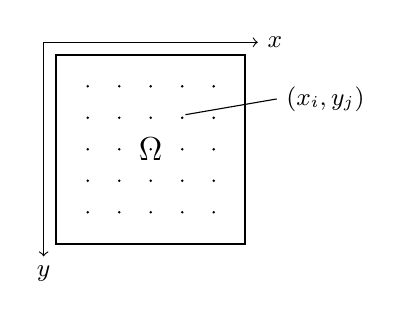
\begin{tikzpicture}[scale=0.8]
          \draw[thick] (0,0) rectangle node[] {\large $\Omega$} (3,3);
          \draw[->] (-0.2,3.2) -- (3.2,3.2) node[right] {\small $x$};
          \draw[->] (-0.2,3.2) -- (-0.2,-0.2) node[below] {\small $y$};
          \foreach \x in {1,...,5}
            \foreach \y in {1,...,5}{
              \draw (\x / 2,\y / 2) node[circle,fill=black,inner sep=0pt] {};
          }
          \draw (2.05,2.05) -- (3.5,2.3) node[right] {\small $(x_i,y_j)$};
        \end{tikzpicture}
      \end{center}
    \end{minipage}
    Dazu soll gelten
    \[\forall (x,y) \in \Omega : ax+by+c \approx f(x,y)\]
    um dieses zu erfüllen wird eine Stichprobe von endlich vielen Punkten $(x_i,y_i)$ aus $\Omega$ gewählt und durch diese ein Gleichungs System gebildet.
    
    \begin{gather*} 
    ax_1+by_1+c \approx f(x_1,y_1)\\
    \vdots \\
    ax_n+by_n+c \approx f(x_n,y_n)
    \end{gather*}
    In Matrix form ergibt sich:
    
    \[\underbrace{\mat{x_1 & y_1 & 1 \\ \vdots & \vdots & \vdots \\ \vdots & \vdots & \vdots \\ \vdots & \vdots & \vdots \\ x_n & y_n & 1}}_{A} \underbrace{\mat{a \\ b \\ c}}_{w} \approx \underbrace{\mat{f(x_1,y_1 \\ \vdots \\ \vdots \\ \vdots \\ f(x_n,y_n)}}_{z}\]
    Die optimale Lösung dieses Problems kann über die \mim{Normalengleichung} berechnet werden.
    
    \[A^T A w = A^T z\]
    
    Dauraus erhält man $w$, somit auch $a$, $b$, $c$ und schlussendlich $v \Rightarrow u = f-v$.\\
    Anschließend wird noch ein Histogram stretching durchgeführt um das finale Bild zu erhalten.
    
    \item[b)] \mim{Polynomiale Regression}:
    Ähnlich zur linearen Regression nun wird hierbei keine affin-lineare Funktion, sondern ein polynom genutzt. Für ein Polynom zwieten gerades kann etwa die Funktion
    \[v(x,y) = ax^2 by^2 cxy+ dx +ey +f\]
    gewählt werden. Wieder entsteht ein Gleichungssytem:
    
    \[\underbrace{\mat{x_1^2 & y_1^2 & x_1y_1 & x_1 & y_1 & 1 \\ \vdots & \vdots & \vdots & \vdots & \vdots & \vdots \\ \vdots & \vdots & \vdots & \vdots & \vdots & \vdots \\ \vdots & \vdots & \vdots & \vdots & \vdots & \vdots \\ x_n^2 & y_n^2 & x_ny_n & x_n & y_n & 1}}_{A} \underbrace{\mat{a \\ b \\ c \\ d \\e \\ f}}_{w} \approx \underbrace{\mat{f(x_1,y_1 \\ \vdots \\ \vdots \\ \vdots \\ f(x_n,y_n)}}_{z}\]

  \item[c)] \mim{Trigonometrisches Polynom}
  Hierbei wird $v$ in den niedrigfrequenten Anteilen von $f$ gesucht.
  
  \begin{center}
    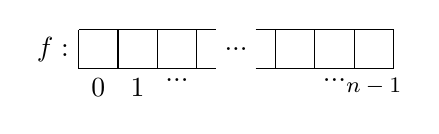
\begin{tikzpicture}
      \draw (0,0.25) node[left] {$f:$};
      \draw[step = 0.5] (0,0) grid (1.75,0.5);
      \draw (2,0.25) node[] {$...$};
      \draw[step = 0.5] (2.25,0) grid (4,0.5);
      \draw (0.25,0) node[below] {$0$};
      \draw (0.75,0) node[below] {$1$};
      \draw (1.25,0) node[below] {$...$};
      \draw (3.25,0) node[below] {$...$};
      \draw (3.75,0) node[below] {\footnotesize $n-1$};
    \end{tikzpicture}
  \end{center}
  
  Es ergibt sich $\hat f$:
  
  \[\hat f_k = \sum_{m=0}^{n-1} f_k \bigl(\underbrace{e^{- i 2 \pi \frac{k}{n}}}_{w_k}\bigr)^m \quad , \ k= 0,1,...,n-1\]
  
  Mittels der FFT (Fast Fourier Transformation) ergibt sich $\hat f$ zu:

  \begin{center}
    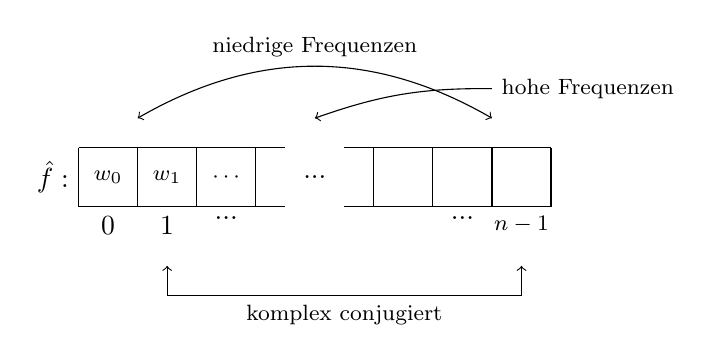
\begin{tikzpicture}[scale=1.5]
      \draw (0,0.25) node[left] {$\hat f:$};
      \draw[step = 0.5] (0,0) grid (1.75,0.5);
      \draw (2,0.25) node[] {$...$};
      \draw[step = 0.5] (2.25,0) grid (4,0.5);
      \draw (0.25,0) node[below] {$0$};
      \draw (0.75,0) node[below] {$1$};
      \draw (0.25,0.25) node[] {\footnotesize $w_0$};
      \draw (0.75,0.25) node[] {\footnotesize$w_1$};
      \draw (1.25,0) node[below] {$...$};
      \draw (3.25,0) node[below] {$...$};
      \draw (1.25,0.25) node[] {\footnotesize$\cdots$};
      \draw (3.75,0) node[below] {\footnotesize $n-1$};
      \draw[<->] (0.75,-0.5) -- (0.75,-0.75) -- node[below] {\footnotesize komplex conjugiert} (3.75,-0.75) -- (3.75,-0.5);
      \draw[<->] (0.5, 0.75) to[bend left] node [above] {\footnotesize niedrige Frequenzen} (3.5,0.75);
      \draw[<-] (2,0.75) to[bend left=10] (3.5,1) node[right] {\footnotesize hohe Frequenzen};
    \end{tikzpicture}
  \end{center}
  Durch entfernen dieser niedrigen Frequenzen ergibt sich $u$.
Ähnliches funktioniert auch in 2D:

    \begin{center}
    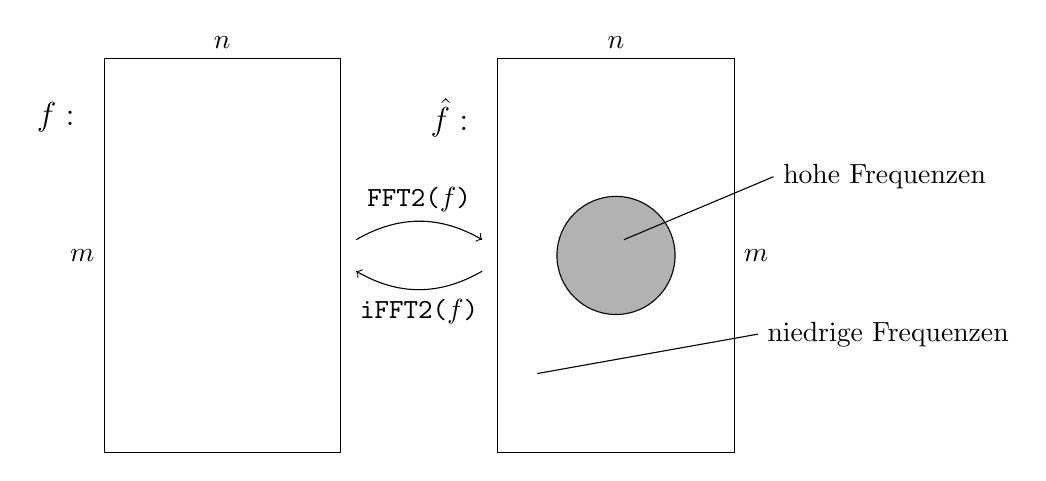
\begin{tikzpicture}[scale=1]
      \draw (0,0) rectangle (3,5);
      \draw (1.5,5) node[above] {$n$};
      \draw (0,2.5) node[left] {$m$};
      \draw (-0.25,4.25) node[left] {\large $f:$};
      \draw[->] (3.2,2.7) to[bend left] node[above] {\tt{FFT2($f$)}} (4.8,2.7);
      \draw[<-] (3.2,2.3) to[bend right] node[below] {\tt{iFFT2($f$)}} (4.8,2.3);
      \draw (5,0) rectangle (8,5);
      \draw (6.5,5) node[above] {$n$};
      \draw (8,2.5) node[right] {$m$};
      \draw (4.75,4.25) node[left] {\large $\hat f:$};
      \draw[fill = black!30] (6.5,2.5) circle (0.75);
      \draw (6.6,2.7) -- (8.5,3.5) node[right] {hohe Frequenzen};
      \draw (5.5,1) -- (8.3,1.5) node[right] {niedrige Frequenzen};
    \end{tikzpicture}
  \end{center}
\end{enumerate}

\section{Thresholding als Variationsproblem}

\begin{enumerate}
\item[geg:] Bild $u: \Omega \to F=[0,1]$ und Schwellenwert $t \in (0,1)$
\item[$\Rightarrow$:]   $\begin{array}{lr}
                            \Omega_0 = \{x \in \Omega : u(x) \leq t \} \to \text{schwarz}  \\
                            \Omega_1 = \{x \in \Omega : u(x) > t \} \to \text{weiß}
                        \end{array} \bigg \}$ soll in ein Variationsproblem umformuliert werden.
\end{enumerate}

Setze dazu:

\begin{equation}\label{eq.9.1}
J(v):=-\int_\Omega (u(x) -t) \C v(x) dx \to \ min
\end{equation}

mit $v \in U:= \bigl \{ v \in \Omega \to \{ 0,1\} \text{ \ (oder $[0,1]$)} \bigr\}$, dies ist jedoch kein Vektorraum.

Die Lösung dieses Problems ist offenbar

\[v = \chi_{\Omega_1}, \ \text{d.h.} \begin{cases}
0, & x \in \Omega_0 \\
1, & x \in \Omega_1
\end{cases} \]

illustiert hier:


\begin{center}
    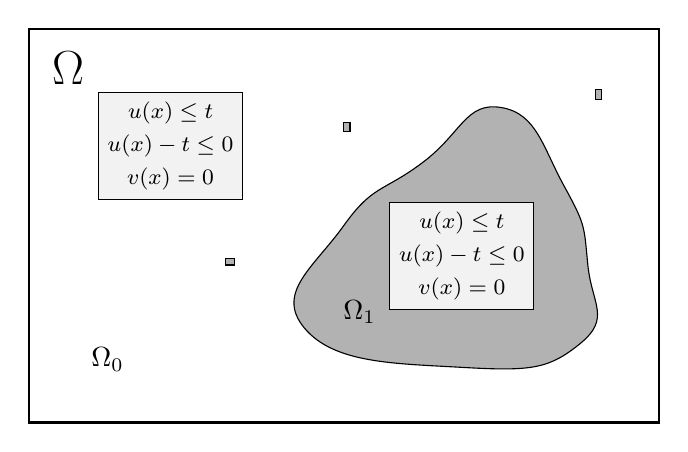
\begin{tikzpicture}
        \draw[thick] (0,0) rectangle (8,5);
        \draw[fill, black!30, draw = black] plot[smooth cycle,tension=0.9] coordinates {(7,1) (7.1,2) (6.8,3) (6,4) (5,3.3) (4,2.5) (3.5,1.2) (5.5,0.7) };
        \draw (0.5,4.5) node[] {\LARGE $\Omega$};
        \draw[white] (0.3, 4.2) -- node[black,below,sloped,style={align=center},draw,fill=black!5] {\footnotesize $u(x) \leq t$ \\ \footnotesize $u(x) -t \leq 0$ \\ \footnotesize $v(x) = 0$} ++(0:3);
        \draw (1,0.8) node[] {$\Omega_0$};
        \draw[] (5.5, 2.8)  node[black,below,sloped,style={align=center},draw,fill=black!5] {\footnotesize $u(x) \leq t$ \\ \footnotesize $u(x) -t \leq 0$ \\ \footnotesize $v(x) = 0$};
        \draw (4.2,1.4) node[] {$\Omega_1$};
        \draw[fill, black!30, draw = black] (2.5,2) rectangle ++(0.11,0.08);
        \draw[fill, black!30, draw = black] (4,3.7) rectangle ++(0.08,0.11);
        \draw[fill, black!30, draw = black] (7.2,4.1) rectangle ++(0.07,0.13);
    \end{tikzpicture}
\end{center}

Diese Herangehensweise ist jedoch kompliziert, um sie zu begründen betrachten wir die Flecken die neben der großen Masse in der obing Illustration zu sehen sind und etwa durch Rauschen entstanden seien könnten. Durch Verallgemeinerung des in \ref{eq.9.1} gegebenen Funktionals können wir die Zerlegung von $\Omega$ in $\Omega_0$ und $\Omega_1$ weniger Anfällig gegenüber Rauschen und sonstigen kleinen Strukturen machen.

Dazu sei

\begin{equation}\label{eq.9.2}
TV(v) = \int_\Omega \abs{\nabla v(x)} dx
\end{equation}

die sogennate \mim{Totalvariation} einer Funktion auf $\Omega$.

Illustration in 1D:

\begin{center}
    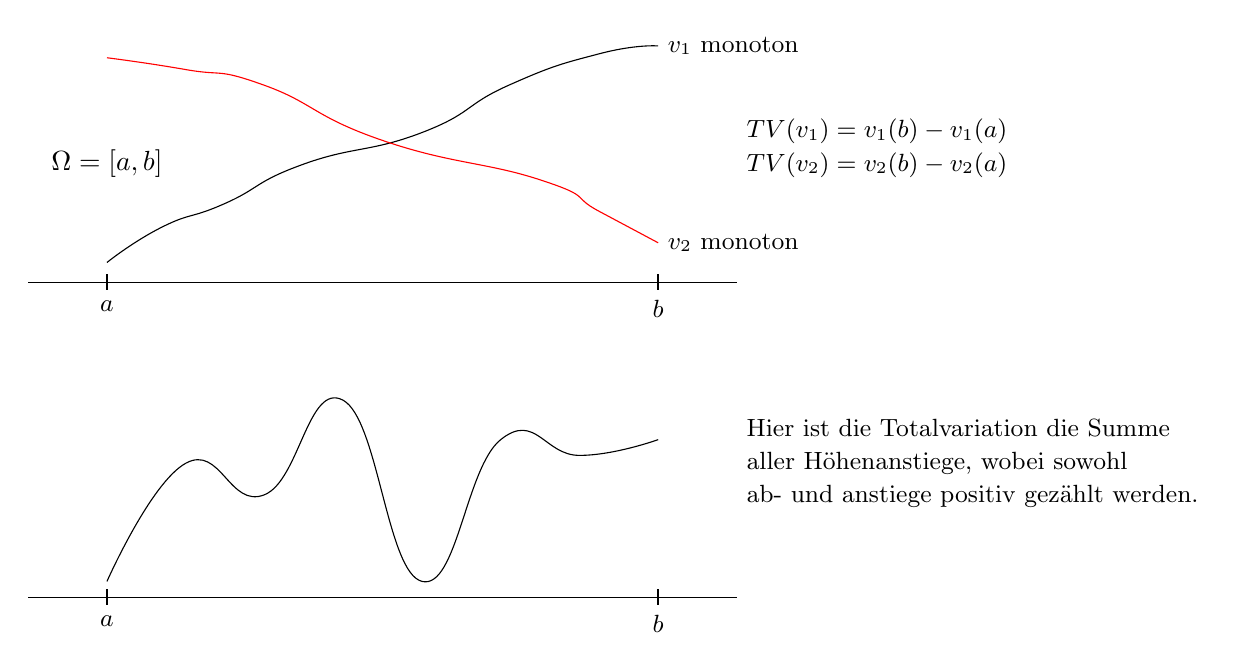
\begin{tikzpicture}
        \draw (0,0) -- (9,0);
        \draw (1,1.5) node[] {$\Omega = [a,b]$};
        \draw plot[smooth,tension=0.9] coordinates {(1,0.25) (1.7,0.7) (2.5,1) (3.5,1.5) (5,1.9) (6.1,2.5) (7.25,2.9) (8,3)} node[right] {\small $v_1$ monoton};
        \draw[red] plot[smooth,tension=0.9] coordinates {(1,2.85) (2,2.7) (3,2.5) (4.5,1.8)  (6.5, 1.3) (7.25,0.9) (8,0.5)} node[black,right] {\small $v_2$ monoton};
        \draw[thick] (1,0.1) -- (1,-0.1) node[below] {\small $a$};
        \draw[thick] (8,0.1) -- (8,-0.1) node[below] {\small $b$};
        \draw (9,1.7) node[style={align=left},right] {\small $TV(v_1) = v_1(b) -v_1(a)$ \\ \small $TV(v_2) = \abs{v_2(b) - v_2(a)}$};
        \draw (0,-4) -- (9,-4);
        \draw plot[smooth,tension=0.8] coordinates {(1,-3.8) (2,-2.3) (3, -2.7) (4,-1.5) (5,-3.8) (6,-2) (7,-2.2) (8,-2)};
        \draw[thick] (1,-3.9) -- (1,-4.1) node[below] {\small $a$};
        \draw[thick] (8,-3.9) -- (8,-4.1) node[below] {\small $b$};
        \draw (9,-2.3) node[style={align=left},right] {\small Hier ist die Totalvariation die Summe \\ \small aller Höhenanstiege, wobei sowohl \\
        \small ab- und anstiege positiv gezählt werden.};
    \end{tikzpicture}
\end{center}

In Abschnitt 11.2 werden wir weiterhin sehen, dass die Totalvariation sich auch auf nicht stetigen Funktionen etwa $\chi_{(0,\infty)}$ berechnen lässt, obwohl für diese der Gradient nicht definiert ist. Für die eben genannte Funktion beträgt die Totalvariationetwa $1$.

Nun in 2D:

\begin{center}
    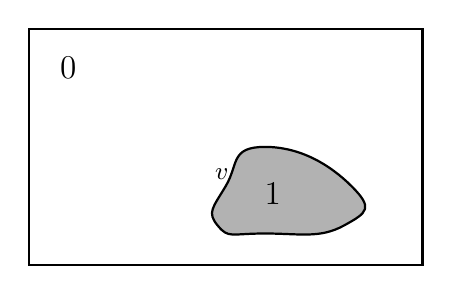
\begin{tikzpicture}
        \draw[thick] (0,0) rectangle (5,3);
        \draw[fill, black!30, draw = black, thick] plot[smooth cycle,tension=1] coordinates {(4,0.5) (4.1,1) (3,1.5) (2.5,1) (2.4,0.5) (3,0.4)};
        \draw (0.5,2.5) node[] {\large $0$};
        \draw (3.1,0.9) node[] {\large $1$};
        \draw (2.45,1.15) node[] {\small $v$};
    \end{tikzpicture}
\end{center}

$TV(v)$ ist hier die Länge der Kante die $\Omega_1$ von $\Omega_0$ trennt.\\
Die Idee ist nun $TV(v)$ als Strafterm zu \ref{eq.9.1} hinzu zu addieren,


\begin{equation}\label{eq.9.3}
\widetilde J(v):= \underbrace{-\int_\Omega (u(x)-t) \C v(x) dx}_{J(x)} + \lambda \C TV(v) \to \ min
\end{equation}
wobei $v \in U$ ist.
Der Effekt dieser Herangehensweise wird nun illustriert.

\begin{center}
    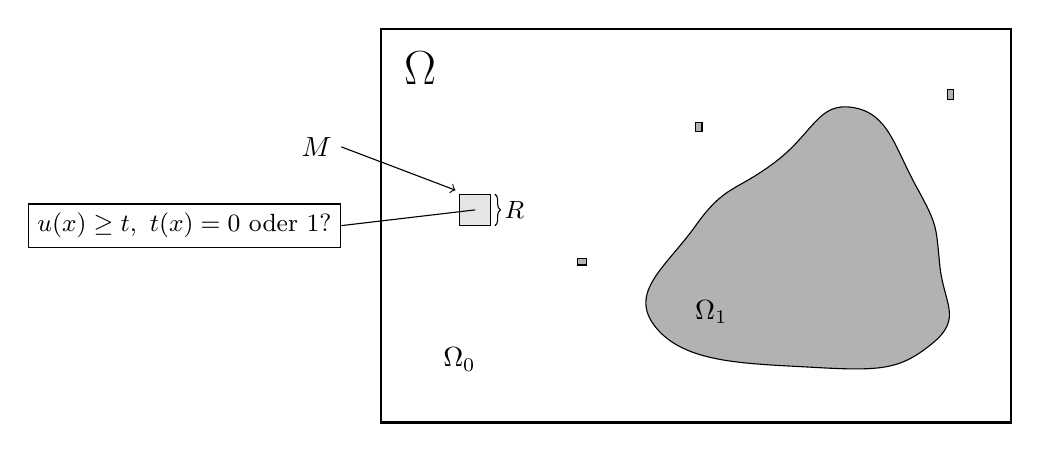
\begin{tikzpicture}
        \draw[thick] (0,0) rectangle (8,5);
        \draw[fill, black!30, draw = black] plot[smooth cycle,tension=0.9] coordinates {(7,1) (7.1,2) (6.8,3) (6,4) (5,3.3) (4,2.5) (3.5,1.2) (5.5,0.7) };
        \draw (0.5,4.5) node[] {\LARGE $\Omega$};
        \draw (1,0.8) node[] {$\Omega_0$};
        \draw (4.2,1.4) node[] {$\Omega_1$};
        \draw[fill, black!30, draw = black] (2.5,2) rectangle ++(0.11,0.08);
        \draw[fill, black!30, draw = black] (4,3.7) rectangle ++(0.08,0.11);
        \draw[fill, black!30, draw = black] (7.2,4.1) rectangle ++(0.07,0.13);
        \draw[fill, black!10, draw = black] (1,2.5) rectangle ++(0.4,0.4);
        \draw[->] (-0.5,3.5) node[left] {$M$} -- (0.95,2.95);
        \draw[] (-0.5,2.5) node[left,draw] {\small $u(x) \geq t, \ t(x)=0$ oder $1$?} -- (1.2,2.7);
        \draw[decorate,decoration={brace,amplitude=2pt}] (1.45,2.9) -- node[right] {\small $R$} (1.45,2.5);
    \end{tikzpicture}
\end{center}

$\begin{array}{cccccccc}
\text{Falls:} & v|_M = 0:&a & +& \lambda \C b \\
\text{Falls:} & v|_M = 1:&a-dR^2 & + &\lambda \C (b+4R)
\end{array} \bigg \}$ Also $M \to 0 \iff 4 \lambda - dR < 0 \iff R > \frac{4 \lambda}{d}$ %??

Das heißt das kleine Segment $M$ wird durch \ref{eq.9.3} \quo{erkannt} falls seine Kantenlänge $R>\frac{4 \lambda}{d}$ ist. Somit können die Abmessung der kleinsten zu segmentierenden Strukturen über $\lambda$ gesteuert werden.

\section{Segmentierung nach Mumford und Shah}

\begin{minipage}{.65\textwidth}
    \begin{enumerate}
        \item[Wieder:] Variationsrechnung
        \item[Diesmal:] Ohne Vorkenntnis des thresholds
        \item[Idee:] Bild zerlegen in \quo{glatte} Teile getrennt durch Sprünge an deren Rändern.
        \item[] \
        \item[geg.:] Bild $u$
        \item[ges.:] Stückweise glattes Bild $v$ mit Randkurve $\Gamma$
    \end{enumerate}
    \begin{enumerate}
        \item[1. Wunsch:] $u \approx v$ auf ganz $\Omega$
        \item[2. Wunsch:] $\nabla v$ klein auf $\Omega \backslash \Gamma$
    \end{enumerate}
\end{minipage}%
\begin{minipage}{0.3\textwidth}
\begin{center}
    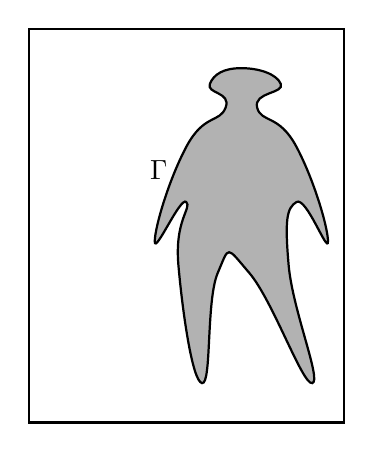
\begin{tikzpicture}
        \draw[thick] (0,0) rectangle (4,5);
        \draw[fill, black!30, draw = black,thick] plot[smooth cycle,tension=0.9] coordinates {(3.6,0.5) (3.3,2) (3.4,2.8) (3.8,2.3) (3.4,3.5) (2.9,4) (3.2,4.3) (2.7,4.5) (2.3,4.3) (2.5,4)  (2,3.5) (1.6,2.3) (2,2.8) (1.9,2) (2.2,0.5) (2.4,1.9) (2.8,1.9)};
        \draw (1.65,3.2) node[] {$\Gamma$};
    \end{tikzpicture}%%(2.7,4)
\end{center}
\end{minipage}

\[\Rightarrow J(v,\Gamma) := \underbrace{\norm{u-v}_{2,\Omega}^2}_{1. \text{ Wunsch}}  + \lambda \underbrace{\norm{\nabla v}_{2,\Omega \backslash \Gamma}^2}_{2. \text{ Wunsch}} \to \ min \]

Wie im letzten Abschnitt \ref{eq.9.2} soll nun noch die Segmentierung sehr kleiner Strukturen vermieden werden, indem man zu $J$ einen entsprechenden Strafterm addiert.

\begin{equation*}
\widetilde J(v,\Gamma) := \norm{u-v}_{2,\Gamma}^2 + \lambda \norm{\nabla v}_{2,\Omega \backslash \Gamma}^2 + \mu \ \text{Länge}(\Gamma) \to \ min
\end{equation*}

Dieses wird \mim{Mumford-Shah-Funktional} (1989) genannt.

\begin{enumerate}
\item[$\lambda$] bestimmt die \quo{Flachheit} von $v$ auf $\Omega \backslash \Gamma$
\item[$\mu$] ist proportional zur Größe der kleinsten zu segmentierenden Struktur.
\end{enumerate}

Die numerische Lösung dieses Problemes ist jedoch sehr kompliziert, da neben $v$ auch die Kurve $\Gamma$ variiert wird, desßhalb existert eine \quo{vereinfachte} Version das dieses Problem approximiert.

Mumford-Shah (1989):

\[\widetilde J(v,\Gamma) := \norm{u-v}_{2,\Gamma}^2 + \lambda \norm{\nabla v}_{2,\Omega \backslash \Gamma}^2 + \mu \ \text{Länge}(\Gamma)\]

Strekalovskiy \& Cremers (2014):

\[\widetilde J(v,\Gamma) := \int_\Omega \left[ \abs{u(x) - v(x)}^2 + \text{min}(\lambda \abs{\nabla c(x)}^2, \mu) \right] dx \]

Die minimierung und $\mu$ simulieren den Sprung an der Randkurve $\Gamma$.

%\chapter{10.Registrierung}

\begin{enumerate}
    \item[geg.:] \begin{align*}
        \text{Referenzbild} & & \text{und} & &  \text{Objektbild}\\
        u_0: \Omega_0 \to F & & \ & & u:\Omega \to F
    \end{align*}
    \begin{center}
        \begin{tikzpicture}
            \draw (-2,0) node[left]{
\includegraphics[scale=0.15]{images/Bild4.png}};
            \draw[->] (-2,0) to[bend left=10] node[above] {?} (2.7,0);
            \draw (2.7,0) node[right]{
\includegraphics[scale=0.15]{images/Bild4skew.png}};
        \end{tikzpicture}
    \end{center}
    \item[ges.:] Transformation/Deformation d.h. $d:\Omega_0 \to \Omega$, die beide Bilder bestmöglich in Einklang bringt.
    \begin{center}
        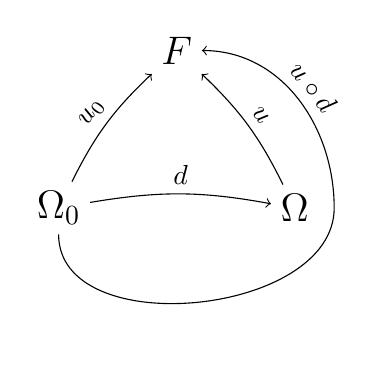
\begin{tikzpicture}
            \draw (-1.5,0) node[](A) {\Large$\Omega_0$};
            \draw (1.5,0) node[](B) {\Large$\Omega$};
            \draw (0,2) node[](C) {\Large$F$};
            \draw[->] (A) to[bend left=10] node[above,sloped]{$d$} (B);
            \draw[->] (A) to[bend left=10] node[above,sloped]{$u_0$} (C);
            \draw[->] (B) to[bend right=10] node[above,sloped]{$u$} (C);
            %\draw[] plot [smooth] coordinates {(A) (2,0) (C)};
            \draw[->] (A) to[out=270, in=270] (2,0) to[out=90,in=0] node[sloped,above]{$u \circ d$} (C);
        \end{tikzpicture}
    \end{center}
\end{enumerate}

Man unterscheidet zunächst in

\begin{enumerate}
    \item[\textbullet] Merkmalsbasierte Verfahren
    \item[\textbullet] Globale Verfahren
\end{enumerate}

\section{Merkmalsbasierte Verfahren}

Hierbei sollen endlich viele \mim{Landmarks}(\mim{Merkmale}) aus $u_0$ und $u$ paarweise in Einklang gebracht werden, hierraus erhält man endlich viele Gleichungen zur Schätzung von $d$. Diese Kontrollpunkte müssen jedoch vorher von Hand bestimmt werden und in den beiden gegebenen Bildern miteinander identifiziert werden, es ist nur schwer möglich dem Computer das Finden dieser Kontrollpunkte beizubringen.

Beispiel.: $d:\R^2 \to \R^2$ linear + Translation, d.h.:

\[ d:\underbrace{\mat{x_1 \\ x_2}}_{p} \mapsto \mat{a & b \\ c & d} \C \mat{x_1 \\ x_2}+ \mat{e\\f}:=\underbrace{\mat{y_1 \\ y_2}}_{q} = \mat{ax_1 + bx_2 +e\\ cy_1 + dx_2 + f} = \underbrace{\mat{x_1 & x_2 & 0 & 0 & 1 & 0\\ 0 & 0 & x_1 & x_2 & 0 & 1}}_{A_p}\C \mat{a\\b\\c\\d\\e\\f}\]

Die zu lösende Gleichung ergibt sich somit zu:

\[A_p \C \mat{a\\b\\c\\d\\e\\f} = q\]

Sind $p_1,...,p_n \in \Omega_0$ und $q_1,...,q_n \in \Omega$ paarweise zusammen gehörende Kontrollpunkte, so kann man $a,b,c,d,e,f$ über das folgende Lineare Ausgleichsproblem schätzen.

\[ \mat{\ \boxed{A_{p_1}} \ \\ \ \boxed{A_{p_2}} \ \\ \cdots \\ \ \boxed{A_{p_n}} \ } \C \mat{a\\b\\c\\d\\e\\f} \approx \mat{\ \boxed{q_1 \vphantom{A_{p_1}}} \ \\ \ \boxed{q_2 \vphantom{A_{p_1}}} \ \\ \cdots \\ \ \boxed{q_n \vphantom{A_{p_1}}} \ }\]

Dieses kann etwa über Normalengleichungen oder QR Zerlegungen geschehen.

\begin{align*}
    n<3&\text{: unterbestimmt}\\
    n=3&\text{: fair}\\
    n>3&\text{: überbestimmt}
\end{align*}

Im selben Stil können quadratische oder höhere Deformationen berechnet werden:

\[d:\underbrace{\mat{x_1 \\ x_2}}_{p} \mapsto \mat{ax_1^2 + b x_1 x_2 + c x_2^2 + d x_1 + e x_2 +f\\ g x_1^2 + hx_1x_2 + ix_2^2 + jx_1 + hx_2 +l} = \underbrace{\mat{y_1\\y_2}}_{q}\]

\[\left(
    \begin{array}{*{12}c}
        x_1^2 & x_1x_2 & x_2^2 & x_1 & x_2 & 1 & 0 & 0 & 0 & 0 & 0 & 0\\
        0 & 0 & 0 & 0 & 0 & 0 & x_1^2 & x_1x_2 & x_2^2 & x_1 & x_2 & 1
    \end{array}
    \right) \C \mat{a\\ \vdots \\ l}\]

Um die 12 gesuchten Parameter hier $a,b, ... ,l$ zu bestimmen werden $n \geq 6$ Kontrollpunkte auf jeder Seite benötigt.

Es gibt auch noch einen anderen Spezialfall der affin-linearen Deformationen, etwa über Dreh-Spiegelungen mit Verschiebung:

\[d: \mat{x_1\\x_2} \mapsto r \C \mat{cos(\varphi) & -sin(\varphi)\\ sin(\varphi) & cos(\varphi)} + \mat{e\\f}=\mat{y_1\\y_2}\]

\[\Rightarrow \mat{y_1\\y_2} = \mat{r \C cos(\varphi)x_1 -r \C sin(\varphi)x_2 + e\\ r \C sin(\varphi)x_1 + r \C cos(\varphi) x_2 + f} = \mat{x_1 & -x_2 & 1 & 0\\ x_2 & x_1 & 0 & 1} \mat{r \C cos(\varphi)\\ r \C sin(varphi)\\e \\ f} \begin{array}{c}
    :=g\\:=h\\ \ \\ \
\end{array}\]

Somit brauchen wir $n \geq 2$ Kontrollpunkte um $g,h,e,f$ zu bestimmen, hierraus können dann $r:=\sqrt{g^2+h^2}$ und $\varphi=arctan(\frac{h}{g})$ bestimmt werden.

\section{Globale Verfahren}

Globale Verfahren benutzen keine Manuell bestimmten Kontrollpunkte und können somit komplett durch einen Computer durchgeführt werden, wiederum wird dieses Problem mittels der Variationsrechnung formuliert.
Hierbei lautet das zu minimierende Funktional:

\[J(d):=\underbrace{D(u_0,u \circ d)}_{\text{\small Datenterm}} + \lambda \underbrace{R(d)}_{\text{\small Regularitätsterm}} \to \ min\]

\begin{enumerate}
    \item Wahl des Datenterms $D$
    \begin{enumerate}
        \item Punktweise Differenz in der$L^1$-Norm:
            \[D(f,g) := \norm{f-g}_2^2 = \int_\Omega \abs{f(x)-g(x)}^2 dx\]
        \item Vergleich der GRauwert-Verläufe
            \[\overline{f} :=\ \frac{1}{\abs{\Omega}} \int_\Omega f(x) dx, \quad \overline{g} := \frac{1}{\abs{\Omega}} \int_\Omega g(x) dx\]
            und dann Vergleich von
            \[\frac{f - \overline{f}}{\norm{f-\overline{f}}_2} \quad \text{und} \quad \frac{g - \overline{g}}{\norm{g-\overline{g}}_2}\]
            über:
            \[\skprod{\frac{f - \overline{f}}{\norm{f-\overline{f}}_2}}{\frac{g - \overline{g}}{\norm{g-\overline{g}}_2}} \in [-1,1]\]

            \begin{enumerate}
                \item[1] bedeutet vollständige Korreliertheit mit gleicher Tendenz
                \item[-1] vollständige Korreliertheit mit entgegengesetzter Tendenz
                \item[0] bedeutet Unkorreliertheit
            \end{enumerate}

            Der sich ergebende Datenterm lautet:

            \[D(f,g) := \skprod{\frac{f - \overline{f}}{\norm{f-\overline{f}}_2}}{\frac{g - \overline{g}}{\norm{g-\overline{g}}_2}}\]

            Diese Verfahren nennt sich \mim{Normalized Crosscorrelation}.
            \item Punktweise Differenzen der Gradienten:
                \[D(f,g) := \norm{f-g}_2^2 = \int_\Omega \abs{\nabla f - \nabla g}^2 dx\]

            \item Vergleich der Gradientnverläufe, also NCC (wie in (b)) von $\nabla f$ und $\nabla g$.
    \end{enumerate}
    Es ist zu bemerken das (a) keine Verschiebung um eine konstante Erkennt, (b) findet sogar Transformationen der Form f=a*g+c.

    \item Notwendigkeit und Wahl des Regularitätsterms.
    Betrachte etwa $\begin{tabular}{|c|c|c|c|}
        \hline
        1 & 2 & 3 & 4\\
        \hline
    \end{tabular} \to \begin{tabular}{|c|c|c|c|}
        \hline
        1 & 4 & 3 & 2\\
        \hline
    \end{tabular}$, diese Zerreißung muss bestraft werden.
    Ansätze:
    \begin{enumerate}
        \item Große Streckungen/Deformationen bestrafen 
            \[R(d) := \int_\Omega\bigl( \abs{\nabla y_1(x)}^2 + \abs{\nabla y_2(x)}^2   \bigr) dx \]
            Hier werden Abbleitung 1. Ordnung benutzt.
        \item Große Krümmungen bestrafen
            \[R(d) := \int_\Omega\bigl( \abs{\Delta y_1(x)}^2 + \abs{\Delta y_2(x)}^2   \bigr) dx \]
            Hier werden Abbleitung 2. Ordnung benutzt.\\
            
            Es können aber auch Ableitungen höherer Ordnungen sowie Kombinationen verwendet werden.
    \end{enumerate}
\end{enumerate}
%\chapter{11.Mathematischer Nachschlag}
Aus mathematischer Sicht sind einige Fragen offen geblieben, etwa:

\newcommand{\D} {
\mathcal{D}
}

\section{Verallgemeinerte Funktionen und Abbleitungen}
Wie differenziert man unstetige Funktionen?

Sei $\D := C_0^\infty(\R^d)$ die Menge (auch ein Vektorraum) der beliebig oft differenzierbaren Funktionen auf $\R^d$ mit beschränktem Träger. Etwa:

\begin{center}
    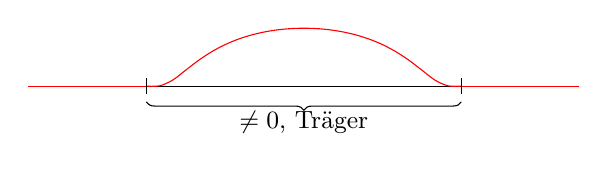
\begin{tikzpicture}
        \draw (-3,0) -- (3,0);
        \draw[scale=2,domain=-0.999:0.999,smooth,variable=\x,red] plot ({\x},{e^(-(1 - abs(\x)^2 )^(-1)});
        \draw[red] (-3.5,0) -- (-0.999*2,0);
        \draw[red] (3.5,0) -- (0.999*2,0);
        \draw (0.999*2,-0.1) -- (0.999*2,0.1);
        \draw (-0.999*2,-0.1) -- (-0.999*2,0.1);
        \draw[decorate,decoration={brace,amplitude=3pt,mirror}] (-2,-0.2) -- node[below] {\small $\neq0$, Träger} (2,-0.2);
    \end{tikzpicture}
\end{center}

Diese Funktion ist:

\[\varphi(x)=g(1- \abs{x}^2)\]

wobei

\[g(t) := \begin{cases}
    e^{\frac{-1}{t}} & ,t>0\\
    0 & ,t\leq 0
\end{cases}\]

Dieses Funktioniert auch im $\R^d$

\def\centerx{2}
\def\centery{-1}

\begin{center}
    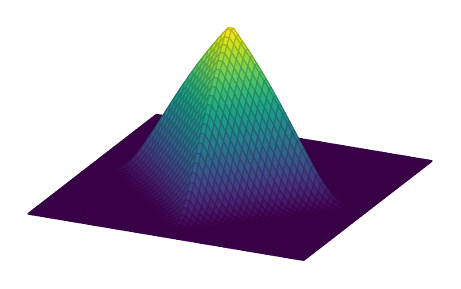
\begin{tikzpicture}[        declare function={
        func(\x) = (\x>0) * e^(-(\x)^(-1)) +
                   (\x<=0) * 0;
      }]

        \pgfplotsset{
            colormap name=viridis,
        }
            \begin{axis}[hide axis,scale=0.75,name=plot1,samples=10]
                \addplot3[surf,domain=-1:1,domain y=-1:1,samples=60]
                    {func(1 - abs(x) - abs(y)))};
                \end{axis}
    \end{tikzpicture}
\end{center}

ist $C_0^\infty(\R^d)$ und hat kompakten Träger.

Sei nun $L^1_{loc}(\R^d)$ die Menge aller Funktionen auf $\R^d$ mit kompaktem Träger für die:

\[\int_K \abs{f(x)} dx < \infty\]

für alle abgeschlossenen und beschränkten Mengen $K \subset \R^d$ gilt.

\begin{center}
    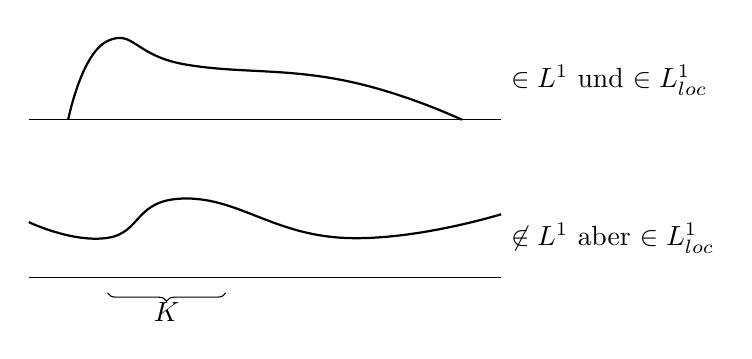
\begin{tikzpicture}
        \draw (-3,0) -- (3,0);
        \draw[thick] plot [smooth, tension = 0.8] coordinates {(-2.5,0) (-2,1)  (-1,0.7) (1,0.5) (2.5,0)};
        \draw (3,0.5) node[right] {$\in L^1$ und $\in L^1_{loc}$};
        \draw (-3,-2) -- (3,-2);
        \draw[thick] plot [smooth, tension = 0.8] coordinates {(-3,-1.3) (-2,-1.5) (-1,-1) (1,-1.5) (3,-1.2) };
        \draw (3,-1.5) node[right] {$\not \in L^1$ aber $\in L^1_{loc}$}; 
        \draw[decorate,decoration={brace,amplitude=3pt,mirror}] (-2,-2.2) -- node[below] {$K$} (-0.5,-2.2);
    \end{tikzpicture}
\end{center}

Die Zweite Funktion ist nicht in $L^1$ da ihr Gesamtintegral nicht endlich ist jedoch ist das Integral über jede endlich Menge endlich, sie hat also keine Pole, somit sie in $L^1_{loc}$.

Für jede Funktion $f \in L^1_{loc}(\R^d)$ bildet 
\begin{equation}\label{eq.11.1}
    \tilde f:\varphi \in \Omega \mapsto \int_{\R^d} f(x) \C \varphi(x) dx \in \R
\end{equation}

ein stetiges lineares Funktional auf $\D$.

Sei nun $\D'$ die Menge aller stetigen linearen Funktionale auf $\D$, also der \mim{Dualraum}. Also ist für jedes $f \in L^1_{loc}$ das Funktional $\tilde f$ aus \eqref{eq.11.1} in $\D'$.

\begin{center}
    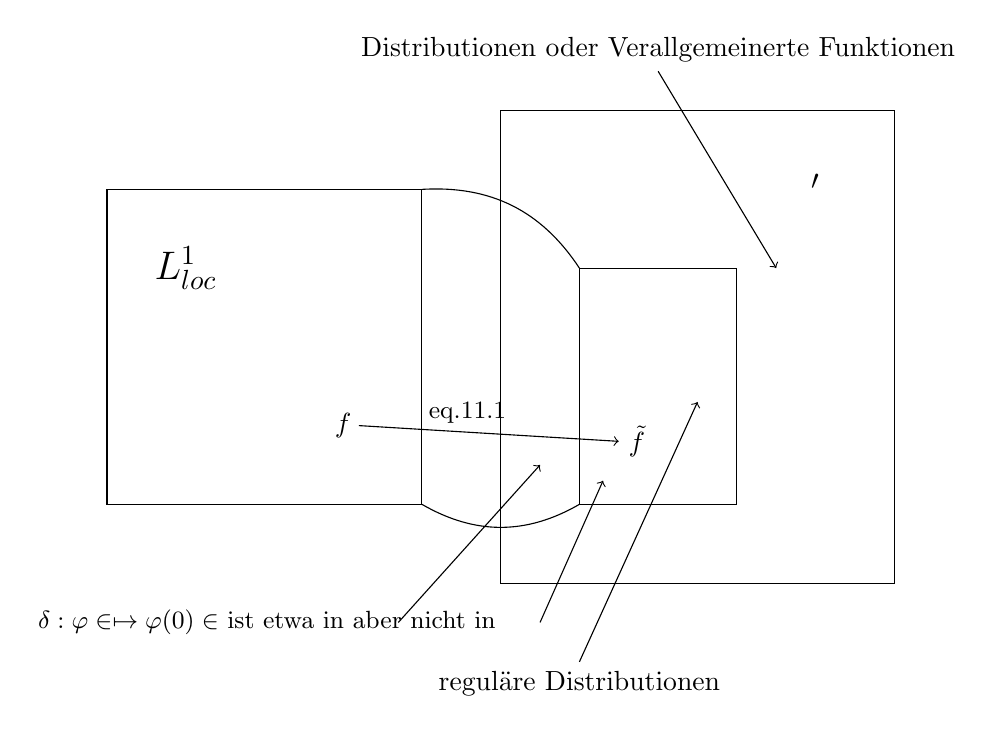
\begin{tikzpicture}
        \draw (0,0) rectangle (4,4);
        \draw (1,3) node[] {\Large $L^1_{loc}$};
        \draw (3,1) node[] {$f$};
        \draw (5,-1) rectangle (10,5);
        \draw (6,0) rectangle (8,3);
        \draw (4,4) to[bend left] (6,3);
        \draw (4,0) to[bend right] (6,0);
        \draw[->] (3.2,1) -- node[above]{\small \eqref{eq.11.1} \ \ \ \ \ } (6.5,0.8) node[right] {$\tilde f$};
        \draw (9,4) node[] {\Large $\D'$};
        \draw[<-] (7.5,1.3) -- (6,-2) node[below]{reguläre Distributionen};
        \draw[<-] (8.5,3) -- (7,5.5) node[above]{\mim{Distributionen} oder Verallgemeinerte Funktionen};
        \draw (-1,-1.5) node[right] {\small $\delta:\varphi \in \D \mapsto \varphi(0) \in \R$ ist etwa in  aber nicht in};
        \draw[<-] (6.3,0.3) -- (5.5,-1.5);
        \draw[<-] (5.5,0.5) -- (3.7,-1.5);
    \end{tikzpicture}
\end{center}

Nun zu den Abbleitungen, sein zunächst $d=1$ und $f \in C^1 \subset L^1_{loc}$, dann gilt für alle $\varphi \in \D$ wobei $[-a,a] \supset supp(\varphi)$:

\[\underbrace{\int_{\R^1} f'(x) \varphi(x) dx}_{f'(\varphi)} = \int_{-a}^a f(x) \phi(x) dx = \underbrace{f(x)\varphi(x)|_{-a}^{a}}_{=0} - \int_{-a}^a f(x) \varphi'(x) dx = -\int_{\R^1} f(x) \varphi'(x) dx = -\tilde f(\varphi')\]

$\Rightarrow$ Für $f \in C^1 \subset L^1_{loc}$ gilt $\tilde f'(\varphi) = - \tilde f(\varphi'), \varphi \in \D$. Wir nehmen dies als Ansatz und setzen:

\begin{equation}\label{eq.11.2}
    F'(\varphi):=-F(\varphi'), \varphi \in \D
\end{equation}

für alle $F\in \D$, genannt Distributionen Abbleitung.

Beispiel:

\begin{center}
    \begin{tikzpicture}
        \draw (-0.4,0) node[left] {$f(x) = \abs{x}$};
        \draw (-0.2,0) -- (4.2,0);
        \draw[thick] (0,2) -- (2,0) -- (4,2);
        \draw (2,-0.1) -- (2,2.3);
    \end{tikzpicture}
\end{center}
Und $F:=\tilde f$ also:

\[F'(\varphi) = -F(\varphi) = - \int_{-a}^a \abs{x} \varphi'(x) dx = - \int_{-a}^0 -x \varphi'(x) dx - \int_0^a x \varphi'(x) dx \]

\[= \int_{-a}^0 x \varphi'(x) dx - \int_0^a x \varphi'(x) dx = \underbrace{x \varphi(x)|_{-a}^0}_{0} - \int_{-a}^0 1 \varphi(x) dx - \underbrace{x \varphi(x)|_0^a}_{0} + \int_0^a 1 \varphi(x) dx\]

\[= \int_{-a}^a sing(x) \varphi(x) dx = \tilde{sign}(\varphi)\]

\begin{center}
    \begin{tikzpicture}
        \draw (-0.4,0) node[left] {$sign(x)=$};
        \draw (-0.2,0) -- (4.2,0);
        \draw (2,-1.3) -- (2,1.3);
        \draw[thick] (2,1) node[left]{\small $1$} -- (4,1);
        \draw[thick] (0,-1) -- (2,-1) node[right]{\small $-1$};
    \end{tikzpicture}
\end{center}

Also insgesamt $F'=\tilde{sign}$

Nun leiten wir die $sign$ Funktion nocheinmal ab:

\begin{align*}
    \tilde{sign}'(\varphi) =& -\tilde{sign}(\varphi') = - \int_\R sign(x) \varphi'(x) dx = - \int_{-a}^a sign(x) \varphi'(x) dx\\
    =&- \int_{-a}^0 (-1) \varphi'(x) dx - \int_0^a 1 \varphi'(x)dx\\
    =&\underbrace{\int_{-a}^0 \varphi'(x) dx}_{\varphi(0) - \varphi(-a)} - \underbrace{\int_0^a \varphi'(x)dx}_{-\varphi(a)+\varphi(0)} = 2 \varphi(0) = 2 \delta(\varphi)\\
    \Rightarrow & \tilde{sign}'=2\delta
\end{align*}

Diese Abbleitung ist jedoch nicht mehr mit einem Element in $L^1_{loc}$ identifizierbar.
Distributionen sind beliebig oft differenzierbar, somit folgt:

\[F^{(k)}(\varphi) = (-1)^kF(\varphi^{(k)}\]

Ein anderes Beispiel in mehr Dimensionen:

Hier ist die Abbleitung definiert über:

\[(D^\alpha F)(\varphi) = (-1)^{\abs{\alpha}}F(D^{\alpha} \varphi), \quad \varphi \in \mathcal{D}, \alpha \in \N^d\]

Für dieses Beispiel ist $d=2$ und $\alpha = \mat{2\\1}$, wobei $\abs{\alpha} = \alpha_1 + ... +\alpha_d$.

\[\Rightarrow D^\alpha = \frac{\partial^{\alpha_1}}{(\partial x_1)^{\alpha_1}}\frac{\partial^{\alpha_2}}{(\partial x_2)^{\alpha_2}} = \frac{\partial^{2}}{(\partial x_1)^{2}} \frac{\partial}{\partial x_2}\]

also

\[(\underbrace{D^\alpha F}_{F_{x_1 x_1 x_2}})(\varphi) = (-1)^{3}F(\varphi_{x_1 x_1 x_2})\]

$\abs{\alpha}=1 \Rightarrow $ eine partielle Abbleitung $\Rightarrow$ Gradient, also Vektor der $1.$ partiellen Abbleitungen.

\subsection{Verallgemeinerter Gradient und Totalvariation}

Für $f:\R^d \to \R$ erwarten wir $\nabla f = \srmatrix{f_{x_1} \\ \vdots \\ f_{x_2}}$

Nun fassen wir jede Komponente $f_{x_1}$ als Distribution auf:

\[\tilde{\nabla f} \coloneqq \mat{\tilde{f_{x_1}}\\ \vdots \\ \tilde{f_{x_d}}}: \mat{\varphi_1 \\ \vdots \\ \varphi_d} \mapsto \underbrace{\tilde{f_{x_1}}(\varphi_1) + \hdots + \tilde{f_{x_1}}(\varphi_1)}_{\in \R}\]

Mit \eqref{eq.11.2} ergibt sich:

\begin{equation}\label{eq.11.3}
    \nabla f(\varphi)=\sum_{k=1}^d \tilde{f_{x_k}}(\varphi_k) \overset{\eqref{eq.11.2}}{=} \sum_{k=1}^d - \tilde{f}\left(\frac{\partial}{\partial x_k} \varphi_k \right) = -\tilde{f} \left( \sum_{k=1}^d \frac{\partial}{\partial x_k} \varphi_k \right) = - \tilde f (div(\varphi)), \ \varphi \in \D^d
\end{equation}

genannt \mim{Distributioneller Gradient}. Das heißt $\tilde{\nabla f}$ ist eine lineare Abbildung von $\D^d \to \R$.

Die Totalvariation von $f \in L^1_{loc}$ ist die Operatornorm dieses Funktionals $\tilde{\nabla f}:(\D^d,\norm{\cdot}_\infty) \to \R$

\begin{equation}\label{eq.11.4}
    TV(f) \coloneqq \underset{\varphi \in \D^d, \norm{\varphi}_\infty = 1}{sup} \bigl| \tilde{\nabla f}(\varphi)\bigr| \overset{\eqref{eq.11.3}}{=} TV(f) \coloneqq \underset{\varphi \in \D^d, \norm{\varphi}_\infty = 1}{sup} \tilde{f}(div(\varphi))
\end{equation}

Für folgende Spezialfälle wird  $TV(\varphi)$ etwas handlicher als in \eqref{eq.11.4}:

\begin{enumerate}
    \item Sei $f \in C^1(\Omega)$, d.h. stetig differenzierbar auf $\Omega \subset \R^d$ und $r \in \R^d$ mit $\norm{r}=1$. Für die Richtungsabbleitung $\frac{\partial f}{\partial r}$ gilt:

    \[\frac{\partial f}{\partial r} = \skprod{\nabla f(x)}{r} \leq \norm{\nabla f(x)} \C \underbrace{\norm{r}}_{1} = \norm{\nabla f(x)}\]

    mit Gleichheit im Falle von $r = \frac{\nabla f(x)}{\norm{\nabla f(x)}}$.
    
    Es ergibt sich:

    \begin{align}\label{eq.11.5}
        TV(f) &= \underset{\varphi \in \D^d, \norm{\varphi}_\infty = 1}{sup} \bigl(\tilde{f_{x_1}}(\varphi_1) + ... + \tilde{f_{x_d}}(\varphi_d)\bigr) \nonumber \\
        &= \underset{\varphi \in \D^d, \norm{\varphi}_\infty = 1}{sup} \underbrace{\int_\Omega f_{x_1}\varphi_1(x) + ... + f_{x_d}(x)\varphi_d(x) dx}_{\skprod{\nabla f(x)}{\varphi(x)}} = \int_\Omega \norm{\nabla f(x)} dx
    \end{align}

    Dabei wird immer $\varphi(x) = \frac{\nabla f(x)}{\norm{\nabla f(x)}}$ gewählt, was zwar im Allgemeinen nicht in $\D^d$ liegt, sich aber beliebig gut approximieren lässt.

    \item Sei $f= \chi_D$ die charakteristische Funktion con $D \subset \Omega \subset \R^d$, wobei $D$ beschränkt sei und stückweise glatten Rand besitzt.
    Dann gilt:

    \[\tilde{\nabla f}(\varphi) \overset{\eqref{eq.11.3}}{=} - \int \chi_D div(\varphi(x)) dx \overset{\text{\small{Gaußscher Integralsatz}}}{=} -\int_{\partial D} \skprod{\varphi(x)}{n(x)} ds(x)\]
    
    wobei $n(x)$ der Normalenvektor an $\partial D$ ist.

    \begin{align}
        \Rightarrow TV(f) =& \underset{\varphi \in \D^d, \norm{\varphi}_\infty = 1}{sup} \int_{\partial D} \skprod{\varphi(x)}{n(x)} ds(x) \nonumber \\
        =& \int_{\partial D}\underbrace{\norm{n(x)}}_{1} ds(x) = \int_{\partial D} 1 ds(x) = \text{Länge}(\partial D)
    \end{align}
\end{enumerate}

\subsection{Existenz und Eindeutigkeit der Variationslösung}
Wann ist ein Minimierungsproblem:

\[J(u) \overset{u \in U}{\longrightarrow}\]

eindeutig lösbar?

\begin{enumerate}
    \item Existenz 
    \[J:U\to \R\]
    Wobei $U$ ein metrischer Raum ist.

    Aus der Analysis ist bekannt, dass stetige Funktionen auf kompakten Mengen ihr Maximum und Minimum annehmen.

    \begin{minipage}[c]{0.49\textwidth}
        
        \begin{center}
            \begin{tikzpicture}
                \draw (-1,0) -- (4,0);
                \draw (0,3) -- (0,-1);
                \draw[{)-*},thick] (0,0) -- (4,0);
                \draw (2,0) node[below] {\small nicht kompakt};
                \draw (-0.2,0) node[below] {\small $0$};
                \draw (4,0) node[below] {\small $1$};
                \draw[scale=0.75,domain=0.25:5.3,thick,smooth,variable=\x,samples=500] plot ({\x},{1/\x});
                \draw[)-,thick] (0,2) -- (4,0.5);
            \end{tikzpicture}
        \end{center}

        \end{minipage}
        \begin{minipage}[c]{0.49\textwidth}
        Nimmt sei Maximum \underline{nicht} an, da $U$ nicht kompakt ist, jedoch ist $f$ stetig.
    \end{minipage}


    \begin{minipage}[c]{0.49\textwidth}
        
        \begin{center}
            \begin{tikzpicture}
                \draw (-1,0) -- (4,0);
                \draw[,thick] (0,0) -- (3,0);
                \draw (1.5,0) node[below] {\small kompakt};
                \draw (0,0.1) -- node[below] {0} (0,-0.1);
                \draw (3,0.1) -- node[below] {1} (3,-0.1);
                \draw[*-(] (0,0.3) -- (2,1.5);
                \draw[*-*] (2,0.3) -- (3,1);
            \end{tikzpicture}
        \end{center}

        \end{minipage}
        \begin{minipage}[c]{0.49\textwidth}
        Nimmt sei Maximum \underline{nicht} an, da $f$ unstetig ist, jedoch ist $U$ kompakt.
    \end{minipage}

    Wir benötigen jedoch nur die Existenz des Minimums, nicht des Maximums, daher reicht im obigen Satz die \mim{Untere Halbstatigkeit}, diese ist für ein $u_0 \in U$ erfüllt falls:

    \[\forall \epsilon > 0 \ \exists \delta: J(U_\delta(u_0)) \subset \left( J(u_0), \infty \right)\]

    Im Vergleich zur gewöhnlichen Stetigkeit:

    \[\forall \epsilon > 0 \ \exists \delta : J(U_\delta (u_0)) \subset U_\epsilon (J(u_0))\]

    Aber auch die Kompaktheit vun $U$ ist nicht oft erfüllt, deshalb definieren wir:
    
    \[S_\alpha  \coloneqq \{ u \in U : J(u) \leq \alpha \}, \quad \text{\mim{Sub-Niveaumenge} zu Niveu $\alpha$} \]

    \textbf{Existenzsatz}: Sei $U$ ein metrischer Raum und 

    \[J:U \to \R\]
    so dass:

    \begin{enumerate}
        \item $J$ unter-halbstetig
        \item $\exists \alpha \in \R : S_\alpha \neq \emptyset$ und kompakt
    \end{enumerate}

    Dann existiert ein Minimierer $u^* \in U$ mit:

    \[J(u^*) \leq J(u) \quad \forall u \in U \]

    \item Eindeutigkeit

    \begin{minipage}[c]{0.34\textwidth}
        
        \begin{center}
            \begin{tikzpicture}
                \draw (0,0) -- (5,0);
                \draw[name path=A] plot [smooth,tension=1] coordinates {(0.25,0.75) (2.5,0.2)  (4.75,1.5)};
                \draw (0.5,0.1) -- node[below] {\small $u$} (0.5,-0.1);
                \draw (4.5,0.1) -- node[below] {\small $v$} (4.5,-0.1);
                \draw[draw =none,name path=B] (0.5,1) -- (0.5,0);
                \draw[draw =none,name path=C] (4.5,1.5) -- (4.5,0);
                \path[name intersections={of=A and B,by=D}];
                \path[name intersections={of=A and C,by=E}];
                \draw[name path = F] (D) -- (E);
                \fill (D) circle[radius = 1.5pt];
                \fill (E) circle[radius = 1.5pt];
                \draw[draw = none, name path = G] (3,1.5) -- (3,0);
                \path[name intersections={of=F and G,by=H}];
                \path[name intersections={of=A and G,by=I}];
                \fill[red] (H) circle[radius = 1.5pt];
                \fill (I) circle[radius = 1.5pt];
                \draw[dotted] (H) -- (3,0);
                \draw (3,0.1) -- (3,-0.1) node[below] {\small $\alpha u + (1- \alpha)v$};
            \end{tikzpicture}
        \end{center}

        \end{minipage}
        \begin{minipage}[c]{0.65\textwidth}
        $J:U \to \R$ heißt \mim{strengkonvex} falls $\forall u,v \in U, \ \alpha \in (0,1)$:

        \[\underbrace{J(\alpha u + (1-\alpha)v)}_{\text{\textbullet}} < \underbrace{\alpha J(u) + (1-\alpha) J(v)}_{\color{red} \text{\textbullet}} \]
    \end{minipage}

    \textbf{Eindeutigkeitssatz}: Falls $J$ strengkonvex ist existiert höchstens ein Minimierer.

    \begin{proof}
        Angenommen, $u^* \neq v^*$ seien Minimierer von $J$, d.h.

        \[\alpha_{\text{min}} \coloneqq J(u^*) = J(v^*) \leq J(u) \quad \forall u \in U\]

        \[\overset{\text{\small str. konvex}}{\Longrightarrow} \forall \alpha \in (0,1) : J(\alpha u^* + (1 - \alpha)v^*) < \alpha J(u^*) + (1-\alpha)J(v^*) = \alpha_{\text{min}} \ \lightning \]

        Dieses ist jedoch ein Widerspruch zur Minimalität von $J(u^*)$ und $J(v^*)$.

    \end{proof}

\end{enumerate}

%\clearpage
%\setcounter{page}{1}


%\appendix 

\end{document}
